\documentclass[AMS,STIX2COL]{WileyNJD-v2}\usepackage[]{graphicx}\usepackage[]{color}
% maxwidth is the original width if it is less than linewidth
% otherwise use linewidth (to make sure the graphics do not exceed the margin)
\makeatletter
\def\maxwidth{ %
  \ifdim\Gin@nat@width>\linewidth
    \linewidth
  \else
    \Gin@nat@width
  \fi
}
\makeatother

\definecolor{fgcolor}{rgb}{0.345, 0.345, 0.345}
\newcommand{\hlnum}[1]{\textcolor[rgb]{0.686,0.059,0.569}{#1}}%
\newcommand{\hlstr}[1]{\textcolor[rgb]{0.192,0.494,0.8}{#1}}%
\newcommand{\hlcom}[1]{\textcolor[rgb]{0.678,0.584,0.686}{\textit{#1}}}%
\newcommand{\hlopt}[1]{\textcolor[rgb]{0,0,0}{#1}}%
\newcommand{\hlstd}[1]{\textcolor[rgb]{0.345,0.345,0.345}{#1}}%
\newcommand{\hlkwa}[1]{\textcolor[rgb]{0.161,0.373,0.58}{\textbf{#1}}}%
\newcommand{\hlkwb}[1]{\textcolor[rgb]{0.69,0.353,0.396}{#1}}%
\newcommand{\hlkwc}[1]{\textcolor[rgb]{0.333,0.667,0.333}{#1}}%
\newcommand{\hlkwd}[1]{\textcolor[rgb]{0.737,0.353,0.396}{\textbf{#1}}}%
\let\hlipl\hlkwb

\usepackage{framed}
\makeatletter
\newenvironment{kframe}{%
 \def\at@end@of@kframe{}%
 \ifinner\ifhmode%
  \def\at@end@of@kframe{\end{minipage}}%
  \begin{minipage}{\columnwidth}%
 \fi\fi%
 \def\FrameCommand##1{\hskip\@totalleftmargin \hskip-\fboxsep
 \colorbox{shadecolor}{##1}\hskip-\fboxsep
     % There is no \\@totalrightmargin, so:
     \hskip-\linewidth \hskip-\@totalleftmargin \hskip\columnwidth}%
 \MakeFramed {\advance\hsize-\width
   \@totalleftmargin\z@ \linewidth\hsize
   \@setminipage}}%
 {\par\unskip\endMakeFramed%
 \at@end@of@kframe}
\makeatother

\definecolor{shadecolor}{rgb}{.97, .97, .97}
\definecolor{messagecolor}{rgb}{0, 0, 0}
\definecolor{warningcolor}{rgb}{1, 0, 1}
\definecolor{errorcolor}{rgb}{1, 0, 0}
\newenvironment{knitrout}{}{} % an empty environment to be redefined in TeX

\usepackage{alltt}

% Packages
\usepackage{amsmath}
\usepackage{amsfonts}
\usepackage{natbib}
\usepackage{subcaption}
\usepackage{xcolor}

% Commands
\definecolor{orange}{rgb}{0.94, 0.59, 0.19}
\definecolor{purple}{rgb}{0.5, 0.0, 0.5}
\definecolor{teal}{rgb}{0, 0.502, 0.502}
\newcommand{\hh}[1]{\textcolor{orange}{#1}}
\newcommand{\kgc}[1]{\textcolor{purple}{#1}}
\newcommand{\kge}[1]{\textcolor{teal}{#1}}
\newcommand{\data}{sine data}

% Set up for ASA data science journal
\articletype{Article Type}
\received{26 April 2016}
\revised{6 June 2016}
\accepted{6 June 2016}
\raggedbottom
\IfFileExists{upquote.sty}{\usepackage{upquote}}{}
\begin{document}

% Paper header (title and authors)
\title{Visual Diagnostics of a Model Explainer -- Tools for the Assessment of LIME Explanations}
\author[1]{Katherine Goode*}
\author[1,2]{Heike Hofmann}
\authormark{Goode and Hofmann}
\address[1]{\orgdiv{Department of Statistics}, \orgname{Iowa State University}, \orgaddress{\state{Iowa}, \country{United States}}}
\address[2]{\orgdiv{Center for Statistics and Applications in Forensic Evidence (CSAFE)}, \orgname{Iowa State University}, \orgaddress{\state{Iowa}, \country{United States}}}
\corres{*Corresponding author. \email{kgoode@iastate.edu}}
\presentaddress{This is sample for present address text this is sample for present address text}

% Abstract and keywords
\abstract[Summary]{The importance of providing explanations for predictions made by black-box models has led to the development of model explainer methods such as LIME (local interpretable model-agnostic explanations) \citep{ribeiro:2016}. LIME uses a surrogate model to explain the relationship between predictor variables from a black-box model and the black-box model predictions in a local region around a prediction of interest. However, the quality of the resulting explanations relies on how well the explainer model captures the black-box model in a specified local region. Here we introduce visual diagnostics to assess the quality of LIME explanations. We propose visualizations for individual explanations, sets of explanations, and comparisons LIME applications with different tuning parameters. We apply the visual diagnostics to a forensics bullet matching dataset to show examples where LIME explanations depend on the tuning parameters and the explainer model oversimplifies the black-box model. Our examples raise concerns about claims made about LIME \citep{ribeiro:2016} that are similar to other criticism found in the literature (\citet{alvarezmelis:2018}, \citet{laugel:2018}, and \citet{molnar:2019}).}
\keywords{LIME, black-box models, interpretability, diagnostics}

% Citation information
\jnlcitation{
\cname{\author{Goode K.}, \author{H. Hofmann}, }
\cyear{2019},
\ctitle{Visual Diagnostics of a Model Explainer -- Tools for the Assessment of LIME Explanations},
\cjournal{Stat Anal Data Min: The ASA Data Sci Journal},
\cvol{volume, number and page}.}

\maketitle



\section{Introduction}

In the field of statistics, there are two main uses for models: inference and prediction. Machine learning models are often used for the latter purpose. While these models have proven to perform well in a wide range of prediction problems, their accuracy generally comes at the cost of interpretability. Most machine learning models are complex algorithms that are good at identifying patterns in the data but lack a simple functional form. The absence of a functional form makes a direct interpretation impractical, and as a result, these models become ``black-box models". Even models with a functional form become difficult to interpret beyond a certain complexity, such as e.g. three-way or higher interactions in logistic regression models.

Throughout this paper, we will make a distinction between interpretability and explanability of models. We define {\it interpretability} as the ability to directly use model parameters to understand the relationships in the data captured by the model: e.g., a linear model coefficient associated with a predictor variable indicates the amount the response variable changes based on a change in the predictor variable. In contrast, {\it explanability} is defined as the ability to use the model in an indirect manner to understand the relationships in the data captured by the model: e.g., partial dependence plots depict the marginal relationship between model predictions and predictor variables \citep{friedman:2001}.

Various methods have been proposed to provide explanations for black-box model predictions \citep{guidotti:2018, mohseni:2018, molnar:2019}. Some are specific to one type of model (e.g. \citep{bau:2017} and \citep{hara:2016}), and others are model-agnostic (e.g. \citep{greenwell:2018} and \citep{strumbelj:2014}). In this paper, we focus on the model-agnostic method of LIME (local interpretable model-agnostic explanations) \citep{ribeiro:2016}.

\subsection{The Importance of Explanability}

The ability to explain a model serves multiple purposes. When a model is fit, explanations help to diagnose the model by checking for relationships between the response and predictor variables. Depending on the training set, some models might pick up on spurious features in the data that are unrelated to the model outcome such as an example described by \citet{ribeiro:2016} where the distinction between huskies and wolves is based on whether there is snow in the background rather than features of the animals.

After a model has been diagnosed, the explanations for the predictions are used to understand the underlying mechanism that produced the data and provide an argument for why the predictions should be trusted. In some areas of application, the ability to be able to explain the results from a model is critical.

The forensics sciences and the heath care industry are two areas that have benefited from machine learning but have an obvious need for explainable predictions. For example, \citet{hare:2016} discuss the use of a random forest model in the forensics sciences to determine whether two bullets were fired from the same gun. \citet{yu:2018} describe how healthcare has advanced through the use of machine learning in ways such as using neural networks to automate medical image diagnoses and implementing Bayesian networks to predict clinical outcomes. In both of these fields, the decisions made based on the results of the machine learning models can greatly impact people's lives. If it is not possible to explain the output from a model, it becomes questionable whether to rely on the predictions to make important decisions.

The European Union has taken the desire to provide explanations for machine learning model predictions a step further. In May 2018, the General Data Protection Regulation (GDPR) went into effect \footnote{https://eugdpr.org/the-regulation/gdpr-faqs/}. The regulation includes a policy that gives the right for individuals affected by decisions made via automated algorithms to understand the logic behind the decisions being made. As \citet{goodman:2016} point out, this regulation has a great effect on the way that machine learning algorithms are used to make decisions. The wording of the policy leaves room for interpretation, but  \citet{goodman:2016} state, ``It is reasonable to suppose that any adequate explanation would, at a minimum, provide an account of how input features relate to predictions, allowing one to answer questions such as: Is the model more or less likely to recommend a loan if the applicant is a minority?"





\begin{figure*}[!htbp]
\begin{knitrout}
\definecolor{shadecolor}{rgb}{0.969, 0.969, 0.969}\color{fgcolor}
\includegraphics[width=\textwidth]{figure/concept-plot-good-1} 

\end{knitrout}
\caption{A conceptual depiction of a faithful LIME explainer model in the immediate neighborhood of a prediction of interest. The predictions from a hypothetical black-box model are plotted against the standardized values of the two predictor variables used to fit the hypothetical model. The diamond shaped points represent the location of a prediction of interest. The size and opacity of the circular points indicate the weight assigned based on the distance to the point of interest computed using the inverse of the Gower distance metric raised to the power of 50. The black lines are a weighted ridge regression model used as an explainer model that reasonably captures the relationship between the black-box predictions and the features in a local region around the point of interest. That is, it is faithful to the complex model and produces a reasonable explanation that Feature 1 plays a more important role in the prediction of interest than Feature 2 since the magnitude of the slope associated with Feature 1 is larger.}
\label{fig:concept-plot-good}

\vspace*{\floatsep}
 
\begin{knitrout}
\definecolor{shadecolor}{rgb}{0.969, 0.969, 0.969}\color{fgcolor}
\includegraphics[width=\textwidth]{figure/concept-plot-bad-1} 

\end{knitrout}
\caption{A conceptual depiction of an unfaithful local explainer model in the immediate neighborhood of a prediction of interest. A ridge regression model is fit to the same black-box model predictions and predictor variables as in \autoref{fig:concept-plot-good}, but the weights are computed using a Gower exponent of 1. The explainer model provides a global approximation of the complex model in regards to the prediction of interest.}
\label{fig:concept-plot-bad}
\end{figure*}

\subsection{Explainer Models}

As a result of the movement to produce explainable predictions, an area of research has emerged on developing ways to explain output from machine learning algorithms \citep{guidotti:2018} \citep{mohseni:2018} \citep{molnar:2019}. Model explainers are one commonly used approach \citep{mohseni:2018}. A model explainer is a method that uses a surrogate model to relate the predictor variables to the black-box model predictions. We will distinguish between the terms of model explainer and explainer model: by \emph{model explainer} we denote the  method for explaining a complex model using a surrogate model, while the \emph{explainer model}, or simply the \emph{explainer}, is the surrogate model.

LIME is one such model explainer \citep{ribeiro:2016}. While some model explainers are focused on understanding a model at the global level, LIME claims to provide local explanations. Additionally, LIME is designed to work with any model and to produce easily understandable explanations \citep{ribeiro:2016}. Conceptually, LIME fits a simple interpretable model, the explainer model,  meant to capture the behavior of the (complex) black-box model in a local region around a prediction of interest. The  simple model then provides interpretable estimates for variables that most influenced the prediction made by the complex model.

\autoref{fig:concept-plot-good} provides a visualization of this conceptual understanding of LIME. The two plots show the predictions from a hypothetical black-box model plotted against the two predictor variables used to fit the hypothetical model. The diamond shaped points represent a prediction  of interest. A Gower distance metric \citep{gower:1971} is used to define locality: the size of the points represent the inverse of the Gower distance as a reflection of the proximity to the prediction of interest. Here, an exponent of 50 is used to emphasize interest in a very local region around the point of interest. A ridge regression model weighted by the proximity values is used as the explainer model. The black-box predictions are used as the response variable, standardized versions of Features 1 and 2 are included as predictor variables. Standardized features allow direct comparisons of the model coefficients. The explainer model is depicted by the black lines in the figure.

The plot on the left of \autoref{fig:concept-plot-good} shows the relationship between the black-box predictions and Feature 1.  Here, the explainer model is plotted with Feature 2 fixed at the observed value of Feature 2 for the prediction of interest. The explainer model captures the relationship in the immediate neighborhood around the prediction of interest  with a slope of 0.068. The plot on the right shows that there is no global or local relationship between the black-box predictions and Feature 2. Here, the explainer model is plotted with Feature 1 set to be the observed value of Feature 1 for the prediction of interest, and it has a small slope of -0.001. The magnitude of the slope associated with Feature 1 is larger than the slope of Feature 2, resulting LIME to report that Feature 1 plays a more important role in the prediction made by the black-box model.

\subsection{Motivation for Diagnosing LIME}

Explainer models are meant to provide clarity to the process of predictive modeling. However, explainer models are an approximation of the complex models and not a direct interpretation. The explanations produced by an explainer model are subject to the quality of the approximation of the explainer to the complex model. This means that explainer models add another layer of complexity to predictive models by requiring yet another model that needs to be relied on for its accuracy.

The choice of exponent in the scenario depicted in \autoref{fig:concept-plot-good} is crucial. High values ensure an up-weight of observations closer to the prediction of interest. Now consider the example depicted in \autoref{fig:concept-plot-bad}. The plots show the same data as \autoref{fig:concept-plot-good}, but the Gower distance metric was raised to the default power used by the \emph{lime} R package of 1. This causes the observations that are further away from the prediction of interest to be given larger weights than before. In \autoref{fig:concept-plot-good}, the explainer model captures the relationship between the black-box predictions in the immediate neighborhood of the prediction of interest. This cannot be said of the explainer model in \autoref{fig:concept-plot-bad}. In addition, the magnitude of the slope (0.011) associated with Feature 2 is larger than that of Feature 1 (0.005). Thus, this explainer model actually provides a misleading explanation that Feature 2 plays a more important role in predicting the observation of interest.

There are various ways in which LIME can fail. One of the biggest difficulties with LIME is determining how to specify a local region \citep{molnar:2019} due to an unclear definition of what a local region means and how to apply LIME to achieve an appropriate local region. \autoref{fig:concept-plot-bad} demonstrates an explainer model that provides misleading explanations due to poorly specified weights. \citet{laugel:2018} show additional examples of undesirable explanations produced by LIME when the local region was chosen inadequately. \citet{alvarezmelis:2018} raise another concern pertaining to the robustness of explanations from LIME and other post-hoc explainers: they find that even small changes in predictor variables can lead to very different LIME explanations. Additionally, LIME relies on a good approximation of the explainer model to the complex model. \citet{ribeiro:2016} acknowledge that ``if the underlying model is highly non-linear even in the locality of the prediction, there may not be a faithful explanation" with a linear regression model as the explainer model.

As a result of the various ways LIME explanations can fail, it is important to assess LIME explanations. In this paper, we lay out the set of claims about LIME made by \citet{ribeiro:2016} and propose visualizations for the assessment of these claims. We have organized our visualizations into three categories:

\begin{itemize}
\item Diagnostics for \emph{Individual Explanations}: Following advice by \citet{wickham:2015}, we visualize the steps taken by LIME to fit the explainer model and plot the model in data space to get a better understanding of the LIME algorithm and an assessment of the claims made at various stages in the creation of the explanation.
\item Diagnostics for \emph{Sets of Explanations}: We visualize a set of explanations associated with a set of predictions to gain insight into the variability in LIME explanations across the feature space and assess the approximations of the explainer models.
\item Diagnostics for \emph{Comparisons of Tuning Parameters}: To assess the tuning parameters used to produce LIME explanations, we visualize sets of explanations associated with the same predictions across applications of LIME using different tuning parameters as defined in \autoref{implementation-visuals}.
\end{itemize}

While LIME has been implemented for image, tabular, and text data, we will only focus on tabular data. For additional simplicity, we will only discuss classification prediction models with a dichotomous response variable and continuous predictor variables. However, the proposed diagnostics are applicable in a wider range of situations.

\subsection{Overview of Paper}

\autoref{background} provides background on LIME including an overview of the LIME algorithm, currently available implementations of LIME, and the claims \citet{ribeiro:2016} make about LIME. We introduce the suggested diagnostic plots in Sections \ref{procedure}, \ref{set-visuals}, and \ref{implementation-visuals}. In \autoref{application}, we  demonstrate the use of the diagnostics to assess LIME explanations for a random forest model fit to a forensics bullet matching dataset. \autoref{discussion} concludes with a discussion on how the examples of the visualizations in this paper find concerns with LIME in regards to the claims made by \citet{ribeiro:2016} that agree with \citet{alvarezmelis:2018}, \citet{laugel:2018}, and \citet{molnar:2019}. Additionally, extensions of the visual diagnostics are discussed.

\section{Background on LIME} \label{background}

LIME was introduced in 2016 by \citet{ribeiro:2016} in an attempt to create a model explainer that produced easily understandable explanations for individual predictions from any predictive model \citep{ribeiro:2016}. The general idea of LIME is to provide an explanation of how a black-box model arrived at a specific prediction for a given observation.

As described by \citet{laugel:2018}, the process performed by LIME can be divided into three steps:

\begin{enumerate}

\item \emph{Data Simulation and Interpretable Transformation}: Simulate a dataset from the original data used to fit the black-box model. Apply a transformation to the simulated data and the prediction of interest that will allow for  interpretable explanations.

\item \emph{Explainer Model Fitting}: Apply the black-box model to the simulated data to obtain predictions. Compute the distance between each of the simulated observations and the prediction of interest. Fit an interpretable model with the black-box predictions from the simulated data as the response, the transformed simulated data as the predictors, and the distances as weights. This model is the explainer model.

\item \emph{Explainer Model Interpretation}: Interpret the explainer model to determine which features played the most important role in the prediction of interest.

\end{enumerate}

\citet{ribeiro:2016} make the following set of claims regarding the performance of LIME:

\begin{itemize}
\item \emph{Interpretability}: The explainer model can be easily interpreted to provide meaningful explanations.
\item \emph{Faithfulness}: The explainer model sufficiently captures the relationship between the complex model predictions and the features in the local region around a prediction of interest to produce explanations that are faithful to the complex model.
\item \emph{Linearity}: By using a ridge regression model as the explainer model, it is assumed that there is a linear relationship between complex model predictions and the features in the local region around a prediction of interest.
\item \emph{Localness}: The explanations produced by LIME are local in regards to a prediction of interest.
\end{itemize}

The assumption of interpretability only depends on the complexity of the model used as explainer model. If the model is too complex to provide meaningful explanations (e.g. there are too many variables in the model), it is clear that the assumption of interpretability is violated. The other three assumptions are not as easy to assess -- for those we suggest the use of diagnostic plots. 

LIME was initially implemented in a Python package\footnote{https://github.com/marcotcr/lime} by the original authors. The adaption to an R package is by Thomas Lin-Pedersen\footnote{https://github.com/thomasp85/lime}. In this paper, we use a forked version\footnote{https://github.com/goodekat/lime} of the development version of the R package \emph{lime} (0.5.1) \citep{pedersen:2020}. The forked version of \emph{lime} allows us to export internal values of the procedure not already exported by \emph{lime}.

\section{Visualizations of an Individual LIME Explanation} \label{procedure}



\begin{figure*}[!t]
\centering
\begin{knitrout}
\definecolor{shadecolor}{rgb}{0.969, 0.969, 0.969}\color{fgcolor}
\includegraphics[width=\textwidth]{figure/sine-plot-data-1} 

\end{knitrout}
\caption{Plots of $x_2$ versus $x_1$ from the training (left) and testing (right) set of the \data \ introduced in Section \ref{procedure}. The true classification boundary is shown as the solid black line in both plots. The color of the training data points represents the value of the observed response variable ($y$). The color of the testing data points represents the random forest probability that an observation belongs to the category of blue ($\hat{y}$). The 18 cases that are misclassified by the random forest are identified by black circles. The prediction of interest to explain is indicated by a diamond.}
\label{fig:sine-plot-data}
\end{figure*}

At a high level, the concept of LIME is relatively simple: an interpretable model is used to approximate a complex model in a local region. In practice, the implementation of LIME is not straightforward, and research is being done to improve the procedure \citep{laugel:2018}. At each step, various decisions have to be made such as the type of distribution to use when simulating data and which distance metric to use to assign weights to the simulated values. It is possible for the procedure to go wrong at any of the internal steps. Without an understanding of or a way to assess the steps, LIME becomes a black-box procedure of its own. To counteract the black-box nature, we suggest the use of visualizations of each step of the LIME algorithm. In this section, we provide example visualizations of the LIME procedure for the creation of an individual explanation.

\paragraph{The \data}

To demonstrate the visualizations, we generate an example dataset that will be referred to as the \data. The \data \ contains 600 observations with three features and one response variable. The features, $x_1$, $x_2$, and $x_3$, are randomly sampled from Unif(-10, 10), Unif(-10, 10), and $\mbox{N}(0,1)$ distributions, respectively. A binary response variable $y$ is  created using a rotated sine curve. In particular, let $x'_1=x_1\cos(\theta)-x_2\sin(\theta)$ and $x'_2=x_1\sin(\theta)+x_2\cos(\theta)$ where $\theta=-0.9$. Then $y$ is defined as
\begin{eqnarray}\label{eq:data}
  y=\begin{cases}
  \mbox{blue} & \mbox{ if } x'_2 > \sin\left(x'_1\right) \\
  \mbox{red} & \mbox{ if } x'_2 \le \sin\left(x'_1\right) \ . %\nolabel
  \end{cases}
\end{eqnarray}
Note that due to the creation of $y$ in this manner, $y$ is dependent on $x_1$ and $x_2$ and independent of $x_3$.

The dataset is divided into a training set of 500 observations and a testing set of 100 observations. A random forest model is fit using the R package \emph{randomForest} (version 4.6.14) \citep{liaw:2002} with the default settings. The model is applied to the testing set to obtain predictions. \autoref{fig:sine-plot-data} shows scatterplots of $x_2$ versus $x_1$ from the training data (left) and the testing data (right). Both plots include the true classification boundary of the rotated sine function plotted as the solid black line. The training data are colored by the observed response variable ($y$), and the testing data are colored by the prediction probabilities from the random forest model ($\hat{y}$).

The random forest model misclassifies 18 points on the classification boundary. These are identified by circles in \autoref{fig:sine-plot-data}. For the visualizations of the steps of the LIME algorithm, we focus on one of these points: the observation with $(x_1, x_2, x_3)$ coordinates of (1.23, 8.47, -0.99) and indicated in \autoref{fig:sine-plot-data} by a diamond.





We apply LIME to the \data \ using \emph{lime} with the default settings. The user is asked to specify the number of features shown in the explanations. Here, we set this value to two, because we expect that $x_1$ and $x_2$ will be the main drivers in the prediction. Note that the complexity of an explanation goes hand in hand with the number of features selected to be included in the explanation. Setting the number of features to a small number will make the explanation simpler but not necessarily more correct.

\autoref{fig:sine-plot-poi} shows the visualization of the explanation produced by \emph{lime} for the prediction of interest. The figure shows that the random forest returned a probability of 0.744 that the observation of interest belongs to category blue {(denoted as the ``label" in the figure). The colored bars indicate the features chosen by LIME and whether they support or contradict a random forest classification of blue. Note that the LIME explanation provides its explanations in form of intervals surrounding the observation of interest. We will discuss this aspect in more detail in Section \ref{step1}. 

The explanation for the prediction of interest depicted in Figure \ref{fig:sine-plot-poi} can be interpreted as follows. A random forest classification of blue is supported by the prediction of interest having a value of $x_2$ that is greater than 4.834, but the prediction of interest having a value of $x_1$ that is greater than -0.302 and less than or equal to 4.844 provides support against a classification of blue. Since the weight associated with $x_2$ has a larger magnitude than the weight associated with $x_1$, LIME explains that the $x_1$ and $x_2$ locations of the prediction of interest provide more support for a random forest classification of blue over red. This explanation agrees with the random forest probability of 0.744 for blue, even though both classify the observation incorrectly.

\autoref{fig:sine-plot-poi} also includes an "explanation fit" value. This value corresponds to the deviance ratio from the R package \emph{glmnet} \citep{simon:2011} for a ridge regression model, or in other words, this is the $R^2$ value associated with the explainer model. In this case, it is 0.21 suggesting that the explainer model is not a good linear fit. However, it is commonly accepted that $R^2$ has limitations for accessing the quality of fit of a model \citep{sapra:2014}, and it should not be the only metric used for assessment of a model. Based on this metric or this plot, it is not yet possible to make an informed assessment of the trustworthiness of the explanation.

We will visualize the steps taken by LIME in creating this explanation to provide insight on why this explanation is returned and to assess its quality. Since the explanation chose the two features, $x_1$ and $x_2$, all of our visualizations will focus on these two features, but they could be extended to include $x_3$ or more features if available. A discussion on the extension of the visualizations to more than two features is included in Section \ref{limitations}. Furthermore, while presenting the visualizations of the procedure, we describe the default procedure options used by \emph{lime} and briefly mention the other available options. More information on the other \emph{lime} options is included in Appendix \ref{lime}.

\begin{figure}[!htbp]
\centering
\begin{knitrout}
\definecolor{shadecolor}{rgb}{0.969, 0.969, 0.969}\color{fgcolor}
\includegraphics[width=0.5\textwidth]{figure/sine-plot-poi-1} 

\end{knitrout}
\caption{Visualization from \emph{lime} of the explanation associated with the prediction of interest from the \data \ produced by the default settings. The probability of 0.744 is the random forest probability in support of a classification of blue. The colored bars indicate that $4.834 < x_2$ supports a random forest prediction of 1 and $-0.302<x_1\le 4.844$ contradicts a random forest prediction of 0. The explanation fit of 0.21 is the $R^2$ value of the explainer model, which indicates that the explainer model has a poor linear fit. Aside of some evidence from the $R^2$ value, it is not clear whether this explanation is reasonable.}
\label{fig:sine-plot-poi}
\end{figure}

\begin{figure*}[!htbp]
\centering
\begin{knitrout}
\definecolor{shadecolor}{rgb}{0.969, 0.969, 0.969}\color{fgcolor}
\includegraphics[width=\textwidth]{figure/sine-plot-step1ab-1} 

\end{knitrout}
\caption{\emph{Training data plot} (left) and \emph{untransformed simulated data plot} (right). Both plots show the 4 quantile bins for $x_1$ and $x_2$ as the vertical and horizontal lines, respectively, overlaid on the \data \ training set colored by the response values (left) and the simulated data colored by the random forest probabilities for category blue (right). The depiction of the random forest predictions for the simulated data shows that the feature space is divided into rectangles of various sizes within which the random forest returns similar probabilities. The intersection of the quantile bins creates a grid that divides the feature space into 16 cells, which is too simple to capture the rectangular pattern of the predictions made by the random forest.}
\label{fig:sine-plot-step1ab}
\end{figure*}



\begin{figure}[!htbp]
\centering
\begin{knitrout}
\definecolor{shadecolor}{rgb}{0.969, 0.969, 0.969}\color{fgcolor}
\includegraphics[width=0.5\textwidth]{figure/sine-plot-step1c-1} 

\end{knitrout}
\caption{\emph{Transformed simulated data plot.} The values of $x'_2$ and $x'_1$ from the simulated data, colored by the random forest probabilities, are plotted behind rectangles representing the interpretability transformed values. The shades of the rectangles represent whether the observation values of $x'_1$ and/or $x'_2$ share the same bin as the prediction of interest. The location of the prediction of interest is denoted by a diamond. This plot shows how the features are simplified by LIME during the interpretability transformation from continuous features to categorical features with two categories each.}
\label{fig:sine-plot-step1c}
\end{figure}

\subsection{Data Simulation and Interpretable Transformation} \label{step1}

The data simulation process involves generating a new set of features based on the training data, applying the complex model to the simulated data to obtain predictions, and transforming the simulated features for ease of interpretation of the explainer model. To understand the progression from the training data to the transformed simulated data that LIME ultimately uses for the explanation, we visualize the three stages in the process. The visualizations corresponding to these stages will be referred to as (a) the \emph{training data plot}, (b) the \emph{untransformed simulated data plot}, and (c) the \emph{transformed simulated data plot}. Examples of these plots with the \data \ prediction of interest are shown in Figures \ref{fig:sine-plot-step1ab} and \ref{fig:sine-plot-step1c}.

The plot on the left in \autoref{fig:sine-plot-step1ab} is the training data plot for the \data \ prediction of interest, which depicts $x_2$ versus $x_1$ from the \data \ training set. The points are colored by the observed response value. The default data simulation in \emph{lime} is done by first dividing each feature in the training data into 4 quantile bins. The black lines in the left plot of \autoref{fig:sine-plot-step1ab} depict the 4 quantile bins for $x_1$ (vertical lines) and $x_2$ (horizontal lines). The quantile bins create a grid that divides the feature space of $x_1$ and $x_2$ into 16 cells. With the inclusion of $x_3$, the quantile bins divide the feature space into 64 cells. In general, the number of cells increases exponentially in the number of features and polynomially in the number of bins. % number of bins to the number of features: $b^f$ that's a polynomial relationship in b
This increase prohibits working with a large number of features or bins. Additionally, an increase in the number of bins may lead to an issue with visualizations of the LIME algorithm due to change blindness. See a further discussion on this issue in Section \ref{limitations}.

By default, \emph{lime} samples 4999 observations for each feature with a probability of 0.25 that an observation is drawn from a quantile bin. The observed feature values of the prediction of interest are appended to the simulated data to create a dataset with 5000 rows. The complex model is applied to the simulated data to obtain predictions. The plot on the right in \autoref{fig:sine-plot-step1ab} is the untransformed simulated data plot, which shows the simulated values of $x_1$ and $x_2$ from the \data \ example denotes as $x'_1$ and $x'_2$. The 4 quantile bin grid used to simulate the data is again depicted by the black vertical and horizontal lines. The points are colored by the random forest prediction probability that an observation is in category blue. The diamond shaped point indicates the location of the prediction of interest in the simulated data. 

The simulated data provide a dense cover of the feature space, which gives insight on how the random forest model creates a prediction based on the $x_1$ and $x_2$ coordinates similar to a partial dependence plot \citep{friedman:2001}. The random forest appears to split the feature space into rectangles of different sizes within which the observations receive similar probabilities. For example, observations with $x_1\in[-10,-2.5)$ and $x_2\in[0,10)$ all have probabilities close to 1. The result is an image of predictions that looks like the rotated sine curve made up of rectangles of varying sizes. The predictions closest to the classification boundary of the curve have random forest probabilities around 0.5.

The random forest predictions depicted with the grid of quantile bins shows how the bins relate to the random forest probabilities. By simulating data using quantile bins, LIME only accounts for the feature space and not the relationship between the features and the response variable. As a result, some of the rectangles created by the quantile bins contain simulated values with similar random forest probabilities, but many of them contain a mixture of probabilities. The quantile bin rectangles are the wrong size to capture the rectangular pattern of random forest predictions. For example, the intersection of quantile bins where $x'_1\in[-5 ,0)$ and $x'_2\in[-5,0)$ is too large to capture the smaller rectangular areas with similar random forest predictions, and the region created by the quantile bins where $x'_1\in[-10,-5)$ and $x'_2\in[5,10)$ is too small to capture the rectangular region in the upper left corner of $x'_1\in[-10,-2.5]$ and $x'_2\in[0,10)$ where the random forest predictions are all approximately 1. The discrepancy between the quantile bin rectangles and the rectangular regions created by the random forest predictions highlights an issue with the LIME claim of faithfulness in this example that will lead to an issue in the interpretation in the explainer model discussed in Section \ref{step3}.

Before the simulated data is used to fit the explainer model, a transformation is applied to the features in the simulated data in an attempt to achieve a representation that will allow for an easy interpretation of the explainer model. We will refer to this as the \emph{interpretability transformation}. With the quantile bin simulation method, the interpretability transformation converts the generated features to binary variables based on whether an observation falls in the same bin as the prediction of interest or not. This transformation is what leads to the intervals used in the LIME explanation shown in Figure \ref{fig:sine-plot-poi}.

The transformed simulated data plot is shown in \autoref{fig:sine-plot-step1c}. The plot shows the simulated values of $x'_2$ versus $x'_1$ as in \autoref{fig:sine-plot-step1ab}, but they are overlaid by rectangles that represent the regions where observations share the same interpretability transformed values. The plot shows two intersecting strips where observations are in the same bin as the prediction of interest for either $x'_1$, $x'_2$, or both. With this transformation, the grid created by the four quantile bins is reduced to 4 categories in the case of two features (or 8 categories accounting for $x_3$).

Overlaying the simulated data with the interpretability transformed values highlights the simplification imposed by the transformation. The rectangle where the prediction of interest is located contains a wide range of random forest predictions from 0.09 to 0.98, but the interpretability transformation groups all of these values into one category. While this transformation  provides easily understandable interpretations, it leads to an extreme over-simplification of the random forest model. This simplification may be one of the reasons underlying the low $R^2$ value associated with the final explainer model and provides further evidence against the LIME claim of faithfulness for this explainer model.

The other simulation methods available in \emph{lime} include quantile bins with a different number of bins, a specified number of equally spaced bins, a kernel density approximation, and a normal distribution approximation. Each of these simulation methods has a corresponding interpretability transformation. See Appendix \ref{lime} for additional information on these other methods. The plots created here are applicable to the other simulation methods.

\subsection{Explainer Model Fitting} \label{step2}

\begin{figure*}[!htp]
\centering
\begin{knitrout}
\definecolor{shadecolor}{rgb}{0.969, 0.969, 0.969}\color{fgcolor}
\includegraphics[width=\textwidth]{figure/sine-plot-step2ab-1} 

\end{knitrout}
\caption{\kge{(Left) \emph{Proximity weights plot}.}\sout{Plots of the weight assignments and feature selection.} The plot \kge{is} \sout{on the left shows} a hex plot \kge{depicting the distribution} of the default \emph{lime} weights (Gower distances raised to the power of 1) assigned to the simulated data prior to the interpretability transformation. \kge{The color of a hexagon represents} \sout{Each hexagon contains} the average of the weights of the observations located within the hexagon. The location of the prediction of interest is \kge{indicated by} \sout{included as} the diamond shaped point. \kge{The black vertical and horizontal lines represent the interpretability transformation boundaries.} The plot shows that the weights increase as the observations approach the prediction of interest, but it is not clear if the region with the largest weights is small enough to provide a valid local interpretation. \sout{Note that the change in weights is not a smooth gradient, which is the result of the value of $x_3$ being taken into account in the calculation of the weight.} \kge{(Right) \emph{Feature selection comparison plot}.} The plot \sout{on the right} shows the features selected by the four feature selection methods in \emph{lime} for the prediction of interest from the \data. The methods produce consistent results since the features of $x_1$ and $x_2$ are chosen by all methods.}
\label{fig:sine-plot-step2ab}
\end{figure*}

\kge{The process of obtaining the explainer model in \emph{lime} involves assigning weights to the interpretability transformed simulated data based on proximity to the prediction of interest, performing feature selection to identify the features to include in the explainer model, and finally, fitting the explainer model. We visualize this process in a series of four plots: (a) \emph{proximity weights plot}, (b) \emph{feature selection comparison plot}, (c) \emph{explainer model prediction plot}, and (d) \emph{explainer model residual plot}. Examples of these plots with the \data \ prediction of interest are shown in Figures \ref{fig:sine-plot-step2ab} and \ref{fig:sine-plot-step2cd}.}

The proximity weights plot for the \data prediction of interest is shown on the left in \autoref{fig:sine-plot-step2ab}. By default, \emph{lime} computes the weights %\sout{for each of the observations in the simulated data}
based on the proximity of the simulated data features prior to the interpretability transformation to the prediction of interest using a Gower distance metric \citep{gower:1971} raised to an exponent of 1. %\kgc{Should I include more details about the Gower distance metric?} \hh{more details here might help with explaining what is going on in the figure below XXX}
The closer an observation is to the prediction of interest, the higher the assigned weight is. \autoref{fig:sine-plot-step2ab} shows a hexplot of the weights assigned to the simulated values from the \data \ for features $x_1$ and $x_2$ with the location of the prediction of interest included as the diamond shaped point. The color shading in each of the hexagons represents the average of the weights for observations located in the hexagon with darker shades representing larger weights. The black lines represent the interpretability transformation boundaries indicating the quantile bins that contain the prediction of interest.

\kgc{Can we talk about the interpretation of this figure? I made some adjustments, but I find this to be a difficult plot to talk about.} \hh{XXX It might become easier if you describe what you are personally looking for in this kind of plot. What would be a surprise, what would be something to react on?}
\sout{Weights are larger the closer an observation is to the prediction of interest, but \hh{interestingly}} \sout{the weights do not decrease in a \sout{smooth}} \hh{\sout{XXX smooth has a mathematical definition. I don't think you are using it that way. What exactly do you mean? decrease consistently in $x_1^2 + x_2^2$? Slow down and explain it precisely.}} \sout{gradient.} \hh{\sout{XXX some of these sentences are very long. They are more effective when shortened.}}, \sout{which is the result of the feature $x_3$ being included in the calculation of the weights.} 
The hexagons in \autoref{fig:sine-plot-step2ab} closer to the prediction of interest have darker shades than those further away, but the weights do not appear to create a tight local region around the prediction of interest in comparison to the ranges of $x_1$ and $x_2$. The darkest shades extend outside of the interpretability transformation region that contains the prediction of interest. This suggests a possible violation of the LIME claim of localness. However, determining whether the assumption of localness is met is difficult, because of a lack of a definition of a local region, and this plot does not include the response variable. The relationship between the response variable and the features would provide a better understanding of a local region that is both large enough for a practical interpretation and small enough to not oversimplify the pattern of the complex model. Since LIME does not account for the response variable in the computation of the weights, we chose to exclude it from our visualization to highlight the ambiguity in a local region. \kgc{I included this last sentence, because otherwise, the sentence before it suggests that we should really include the response variable in the visualization. I can't figure out a good way to include the response variable without the figure becoming too overwhelming.} \hh{sure, it sounds good}

\hh{XXX how do these plots survive a move to higher dimensions? Given that even in the sine example the weights don't seem to show a 2d relationship, I am doubtful.} \kgc{I don't really understand your comment here. Especially since I created visualizations of the weights in "higher dimensions" in the appendix (\autoref{fig:app-plot-step2a}).} \hh{I think this ties into what the purpose of the plots is - once that is clear, it's easier to determine how well the plots keep their purpose in higher dimensions.} 

\hh{A point of criticism for LIME might also be that the weights do not regard importance of features, but are determined ahead of time. If weights were included in the modelling process in form of a parameter better local regions might be achievable.} \kgc{This is an interesting thought. However, would it be reasonable to perform feature selection without the weights? Then feature selection would be done without trying to account for the local region.}

After the weights are computed, feature selection is performed. \autoref{fig:sine-plot-step2ab} is the feature selection comparison plot for the \data \ example. \emph{lime} offers several ways to perform feature selection. If the user has requested 6 or less features be selected, \emph{lime} performs feature selection by first fitting a weighted ridge regression model with the complex model predictions from the simulated data as the response variable, the interpretability transformed simulated data features as the predictor variables, and the proximity measures as the weights. Then forward selection is used to select the features. The feature selection comparison plot includes the features selected by the default \emph{lime} method and three other methods to determine if the features selected are dependent on the method.
%\sout{used for the \data \ prediction of interest, we applied all four feature selection methods to the prediction of interest in the \data. for each of the methods.}

In the case of the \data \ prediction of interest, all methods selected features $x_1$ and $x_2$. This indicates that the methods are consistent in selecting the same features for the prediction of interest. If the selected features were not the same across methods, additional work may be required to determine which method should be used to return the LIME explanation. The application of LIME to the \data \ example will proceed with the default feature selection method of forward selection.



\begin{figure*}[!htbp]
\begin{knitrout}
\definecolor{shadecolor}{rgb}{0.969, 0.969, 0.969}\color{fgcolor}
\includegraphics[width=\textwidth]{figure/sine-plot-step2cd-1} 

\end{knitrout}
\caption{(Left) \emph{Explainer model prediction plot}. The explainer model divides the feature space associated with $x_1$ and $x_2$ into four categories. This plot shows the four categories and the prediction from the explainer model associated with each category. The division of the feature space into four prediction regions  is clearly a major simplification of the random forest model. (Right) \emph{Explainer model residual plot}. The plot shows the residuals versus the predicted values  from the \kge{prediction of interest} explainer model. \hh{XXX Jitter is not added - points are jittered} Jitter has been added to the x-direction. There is an upward trend in the residuals as the explainer model predictions increase, which suggests a violation of the linearity assumption of the ridge regression model.}
\label{fig:sine-plot-step2cd}
\end{figure*}

Finally, the explainer model is fit. \emph{lime} uses a weighted ridge regression model as the explainer model. Similar to the feature selection step, the complex model predictions from the simulated data are the response variability and the proximity measures are the weights, but only the interpretability transformed features identified during feature selection are used as the predictor variables. In the case of the \data, the explainer model predictor variables are the interpretability transformed versions of $x_1$ and $x_2$. The predictions from the explainer model associated with the \data \ prediction of interest are visualized in the explainer model prediction plot shown in \autoref{fig:sine-plot-step2cd} \kge{(left)}. Recall that the interpretability transformed features are binary variables. In the ridge regression model, the transformed features act as indicator variables for whether an observation falls in the same quantile bin. Since the \data \ explainer model contains 2 features, the explainer model prediction plot shows four colored regions indicating the four possible predictions produced by the model. In general, the \emph{lime} explainer model would produce $2^k$ prediction regions for $k$ indicator variables. \hh{XXX generally it would be $2^k$ for $k$ indicator functions - this is very small until it becomes unfeasible. So generally, it is doubtful that it is ever actually useful. XXX} \kgc{I'm not quite sure what you are getting at here: the visualizations or the explainer model in general? Is the last sentence I added enough to address your comment?} \hh{We can talk about this - my comment is again along the lines of bins being too large and too small at the same time. to only have 2 predictions for each variable is ridiculously simple until the number of features is large and $2^k$ becomes computationally unfeasible to manage.}

%\sout{The explainer model predictions mimic the random forest prediction.} \hh{\sout{XXX given that the random forest predictions are used, that is what the explainer model is supposed to do? You could put a bit more opinion in this paragraph.  XXX}}

%\sout{For example, the region where $5\le x_2$ has a prediction of approximately 0.8, which is reasonable considering that many of the observations from the simulated data in this region have a random forest prediction between 0.75 and 1 as seen in} \autoref{fig:sine-plot-step1ab}. \sout{However, by providing only one prediction,}

Compared to the relationship between the random forest predictions and the features of $x_1$ and $x_2$ shown in Figure \ref{fig:sine-plot-step1ab}, the explainer model is a major simplification of the random forest model. Consider the region where the prediction of interest is located. The explainer model provides a single prediction of 0.65 for the entire region as a summary of random forest predictions ranging from 0.09 to 0.98 with a mean and standard deviation 0.68 and 0.2, respectively. The random forest prediction for the prediction of interest is 0.74. Consider that the mean prediction from the random forest (0.68) agrees with the explainer model prediction (0.65) as is expected due to the nature of the explainer model used, but the random forest prediction associated with the case of interest (0.74) is about a half \sout{1} standard deviation away from the mean. \kgc{After reading the previous sentence again, I'm wondering if the next sentence is too dramatic. (Especially since I had made a mistake with the standard deviation.)} \hh{XXX how about we put a 'suggest' into it?} The difference between the explainer model and random forest predictions for the case of interest along with the amount of variability in the random forest predictions in this region makes it clear that the explainer model is simplifying the random forest model too much and violating the assumption of faithfulness. 

%\hh{\sout{avoid these parenthetic intros ... people listen/reader see the beginning of a sentence. Put emphasis on the important ideas you want to get across.}} \sout{With the explainer model fit, we are able to assess the linearity assumption. To do this, we consider a residual plot shown in} \autoref{fig:sine-plot-step2cd} (right).

In order to assess the claim of linearity, we use one of the most basic diagnostics in a statistician's tool box and draw a residual plot for the explainer model. The right plot in \autoref{fig:sine-plot-step2cd} shows residuals on the y axis and explainer model predictions on the x axis. \hh{The points along the $x$ axes have been jittered} to \hh{ease the effect of} the over-plotted points in the visualization. The discretization of the feature space to four categories can again be see in this plot. There is a clear increasing trend in the residuals as the explainer model predictions increase. \hh{XXX the `clear' is repeated} This \kge{is a clear of} \sout{suggests} \hh{\sout{suggests is very nice to lime ... clear indication?}} a violation of the linearity assumption with the ridge regression model. 

\kgc{Do you think there is anything else that should be said about the figures in this section? It feels like we need something else, but I'm not quite sure what.}\hh{I'm not sure what else there could be said about these visualizations in particular, but a paragraph on limitations/general use would be good.}

\emph{lime} offers several other options for fitting the explainer model. Instead of a Gower distance to compute the weights, an exponential kernel can be used. As touched on in Figure \ref{fig:sine-plot-step2ab}, \emph{lime} offers the methods of highest weights, LASSO path, and tree for feature selection, and a different default method is used if more that 6 features are specified to be selected. More details about these options are included in Appendix \ref{lime}.

\begin{figure*}[!htp]
\begin{knitrout}
\definecolor{shadecolor}{rgb}{0.969, 0.969, 0.969}\color{fgcolor}
\includegraphics[width=\textwidth]{figure/sine-plot-step3ab-1} 

\end{knitrout}
\caption{\emph{Explanation plot} (left) \hh{I very much like the explanation plot. but is there a way to get rid of the actual values of the features for the interval and describe instead what it is? 2nd quartile, 3rd quartile? Visually, if the plots don't have the same height you would emphasize that the left and the right plot show different things. You could e.g. move the legend on the left side underneath the bars. That squishes the bars to a different size from the quantiles on the right.} and \emph{complex and explainer model comparison plot} (right). The explanation plot depicts the estimated parameters from the explainer model. The lengths of the bars represent the absolute values of the coefficients, and the colors of the bars represent the coefficient values. Since the magnitude of the coefficient associated with $x_2$ is longer than that of $x_1$, the explanation suggests that $x_2$ has more of an effect on the random forest prediction of interest than $x_1$ does. The explainer model comparison plot shows the simulated data colored by the random forest probabilities and sized by the assigned LIME weights. The prediction of interest is shown as the diamond shaped point. The quantile bins associated with $x_1$ and $x_2$ are depicted by the solid lines. The color of the line indicates whether the explainer model supports a prediction of 'blue' (blue line) or supports a prediction of 'red' (red lines). This figure shows that the quantile bins are not flexible enough to capture the relationship between the random forest predictions and the $x_1$ and $x_2$ values.}
\label{fig:sine-plot-step3ab}
\end{figure*}

\subsection{Explainer Model Interpretation} \label{step3}

\kgc{I made a handful of adjustments to this section including switching out the zoomed in plot for my preferred version of the \emph{lime} plot of the explanation. I also tried to adjust the interpretations based on your comments. See what you think...}

\hh{XXX one thing that the reader should be reminded of is that LIME is actually fitting an explainer model for each observation of interest, i.e. we have not just an explainer model $g$ but a whole family of models. In the example we have 16 possible structures, one of which you are investigating more closely.} \kgc{I'm not sure that we need to remind them of this here. The whole point of this section is that we are focusing on the explainer model for one observation. I'm hoping by this point, they have it locked in their mind that all of this section is focused on one explanation. If not, maybe we need to go back and make it more clear through it. I it would be better to include this reminder at the start of the next section. That could be a really nice was to set up the scenario of diagnostic plots for a set of explanations.} 
\hh{I can see your point, but I still think that it is important to keep it in the back of the readers mind that an explainer model is only valid for a single prediction and any interpretation needs to be repeated. }

The main idea behind LIME, is to interpret the coefficients of the explainer model  to identify the feature(s) of importance in the prediction of interest. To aid in the interpretation and ultimately the assessment of the explainer model, we visualize the coefficients from the explainer model and alongside a visualization of the complex model predictions with the explainer model. We will refer to these plots as (a) the \emph{explanation plot} and (b) the \emph{complex and explainer model comparison plot}, respectively. Examples of these plots with the explanation for the \data \ prediction of interest are included in Figure \ref{fig:sine-plot-step3ab}.

The plot on the left in Figure \ref{fig:sine-plot-step3ab} is the explanation plot for the prediction of interest from the \data. This plot is an extension of the visualization of the LIME explanation from the \emph{lime} R package shown in Figure \ref{fig:sine-plot-poi}. Similar to the plot from \emph{lime}, we include the coefficients from the explainer model for the interpretability transformed features of $x_1$ and $x_2$, but we depict the magnitude of the coefficients by the length of the bars as opposed to the coefficient value for ease of comparison between the lengths of the bars. We represent the coefficient value by the colors of the bar, so that it is still possible to understand which . We also include the intercept to remind the viewer of its role in the ridge regression model. The axis labels we use are meant to be more informative than those of the \emph{lime} plot such as "explainer model coefficient magnitude" as opposed to "weight". \hh{XXX I like the changed plots!}

We can use the explanation plot to interpret the explainer model in terms of a ridge regression coefficients. The intercept, 0.47, is the predicted random forest probability for observations that are not in the same $x_1$ or $x_2$ quantile bins as the prediction of interest. The coefficients are interpreted as the amount that the average random forest probability increases/decreases if an observation falls in the same bin as the prediction of interest. In this example, the average random forest probability that an observation is in category 'blue' increases by 0.31 if an observation falls in the same $x_2$ quantile bin as the prediction of interest (i.e. the third quantile), and the average random forest probability that an observation is in category 'blue' decreases by 0.13 if an observation falls in the same $x_1$ quantile bin as the prediction of interest (i.e. the fourth quantile). Because the magnitude of the coefficient associated with $x_2$ is larger, it indicates that $x_2$ affects the random forest prediction more than $x_1$. Note that if a different simulation method is used when applying LIME, the interpretation of the explainer model can change. See Appendix \ref{lime} for more details.

%\sout{\hh{In a} ridge regression model, the interpretation of the coefficients  depends on the interpretability transformation applied.} \hh{\sout{XXX something went wrong in the previous sentence ... of the transformation?}} \hh{\sout{XXX this would be a good place to tie in the example.}} \sout{In the case of bin based samples, $z'_{j,i}=1$ if feature $j$ is in the same bin as $x^*_j$.} \sout{Thus, the coefficient $\hat{\beta}_j$ can be interpreted as the amount that the response probability increases/decreases if an observation falls in the same bin as $x^*_j$. Thus, the magnitude of the coefficient \hh{XXX is supposed to describe}  the importance of the feature. \hh{XXX write this out in words} That is, $\left|\hat{\beta}_j\right|>\left|\hat{\beta}_{j'}\right|$ indicates that feature $j$ has more effect on the prediction than feature $j'$. \hh{XXX This can go into the appendix?} The magnitudes of the coefficients are used to order the $P$ features in terms of importance in the prediction associated with $x^*$.}

%\sout{In the case of the prediction of interest from the \data, we can interpret the explainer model as follows. \hh{XXX Instead of writing out numbers, I would suggest to describe the bins in words lowest quartile, third, second, top quartile, ...  XXX} For an observation that has a value of $x_1$ that is greater than round(x1_lower, 1) and less than or equal to round(x1_upper, 1), the probability that the observation is predicted to be in category blue decreases by abs(round(sine_b1, 1)), and if an observation has a value of $x_2$ greater than round(x2_lower, 1), the probability that the observation is predicted to be in category blue increases by abs(round(sine_b2, 1)). Since the magnitude of the coefficient associated with $x_2$ is larger, it indicates that $x_2$ plays a more important role of the random forest prediction than $x_1$. The figure produced by \emph{lime} shown in} \autoref{fig:sine-plot-poi} \sout{shows a visualization of the coefficients from the explainer model to provide a high level visualization of the LIME explanation.}

The plot on the right of Figure \ref{fig:sine-plot-step3ab} is the complex and explainer model comparison plot for the prediction of interest from the \data. This figure shows the relationship between the random forest model and the LIME explainer model. The random forest model is represented by the simulated values of $x'_2$ versus $x'_1$ colored by the random forest predictions. The explainer model is represented by the solid horizontal and vertical line identify the boundaries of the quantiles that contain the prediction of interest. The color of the lines represents whether the coefficient of the corresponding indicator variable in the explainer model supports a random forest prediction of 'blue' (blue lines) or not (red lines). Additionally, the size of the simulated data points represents the proximity weight used to fit the ridge regression explainer model. The prediction of interest is represented by the diamond shaped point.

%\hh{\sout{XXX tighten by focusing on the results rather than the process}}
%To provide insight into this explainer model produced by \emph{lime}, we created an additional visualization that incorporates the simulated data
%\sout{To provide a direct comparison of the explanation produced by the explainer model with the complex model. The plot on the left in} \autoref{fig:sine-plot-step3ab} \sout{is a plot of the simulated values of $x'_2$ versus $x'_1$ colored by the associated random forest probability and sized by weight \hh{XXX define weight more precisely }.  This part \hh{do you mean the weights by 'this part'? } of the visualization represents the complex model. The prediction of interest is shown by the diamond shaped point. The explainer model is represented by the red and blue solid lines \hh{XXX how do you come up with the colors for the lines?}, which are the bins from the ridge regression model associated with $x'_1$ and $x'_2$. A close up of the intersection of the bins is included as the plot on the right.}

%\sout{These figures show the relationship between the random forest model and the LIME explainer model.} 
By juxtaposing the random forest predictions and the explainer model boundaries, we are able to assess the faithfulness and localness of the explainer model. First consider the claim of localness. The weights remain relatively high  outside of the intersection of the two quantile bins suggesting that the LIME explanation is highly influenced by points outside of the bin containing the prediction of interest. While it is still difficult to say whether or not the claim of localness has been violated, it is possible to say that the weights assigned to the simulated data do not agree with the local region assigned by the intersection of the quantile bins. Next, let us consider the claim of faithfulness. 

%\sout{The $x_2$ bin contains a majority of random forest probabilities greater than 0.5, whereas the $x_1$ bin contains mostly random forest probabilities less than 0.5.}
Within the intersection of the $x'_1$ and $x'_2$ quantile bins, there appears to be more random forest probabilities above 0.5. This indicates why the magnitude of the coefficient associated with $x_2$ is larger than that of $x_1$. However, the pattern of the random forest predictions in this plot suggest that a better explanations for this prediction exist. One example of a better explanation would be to say that the prediction of interest received a random forest prediction greater than 0.5 since the observation of interest falls in the region where $x_1$ is less than 2.5 and $x_2$ is greater 4.5. Another more localized explanation would be to say that  the region around the prediction of interest shows that observations with $-0.3 < x_1 <= 2.5$ and $4.8 < x_2 <= 8.75$ are all assigned probabilities greater than 0.5. The procedure implemented by LIME is not flexible enough to capture either of these explanations. %\sout{The LIME algorithm overlooked this region, which provides a more detailed explanation of the prediction made by the random forest for the case of interest. This explainer model} \hh{\sout{is too simplistic to meet the criteria of faithfulness or localness.}} 

The visualizations within this section have repeatedly shown issues with a definition of locality and an oversimplification of the random forest model. LIME does provide an explanation for the prediction of interest, which makes sense based on the quantile bins used. However, the visualization of the complex and explainer model comparison plot solidifies the understanding that better explanations for the prediction of interest exist. \kgc{What do you think of this conclusion? I'd like to neatly wrap up the procedure visualizations in some way like this, but I'm not quite sure what to say.}\hh{that sounds good}

\subsection{\kge{Visualizations in Higher Dimensions}} \label{limitations}

\kgc{Help! I don't know how much information to include here. Right now I have it down to one paragraph...}

\hh{By tightening the work I did not mean to cut paragraphs or ideas. The ideas are good, but they need tighter, in the sense of sharper, arguments. }

\kgc{Need to work this in}: \hh{In terms of limitations of the visualizations: first two features span the x and y axis, additional features can be used for faceting. four features is completely feasible, beyond that the visualization might not work as well. The number of bins should be in the single digits. A large number of small multiples \citep{Becker:1996gy} needs a strong signal in the data to be effective - otherwise the visualization might be affected by change blindness \citep{simonsChangeBlindness1997, review19}. }

The \data \ provide a \kge{neat} \kge{very clean} example of how to use the proposed visualizations to assess a single LIME explanation \kge{with two features. Once the number of features is greater than 3, adjustments will need to be made to the plots. In this case, multiple plots will be required to visualize the majority of the steps in the LIME procedure. Reasonable extensions would be scatterplot matrices or the use of faceting. \hh{XXX this is too vague: when do you use scatterplot matrices, what is the advantage of faceting. Make your solutions more concrete by discussing them as well as their limitations. }
In the case of faceting, the} \hh{first two features} \kge{can} \hh{span the x and y axis,} \kge{and} \hh{additional features can be} \kge{used as the facets.} We have included some examples of such plots in Appendix \ref{scatter-plots} that take into the feature $x_3$ from the \data \ in the visualization of the LIME procedure. 

\hh{\sout{In terms of limitations of the visualizations: first two features span the x and y axis, additional features can be used for faceting. four features is completely feasible, beyond that the visualization might not work as well. The number of bins should be in the single digits. A large number of small multiples (reference to Cleveland?) needs a strong signal in the data to be effective - otherwise the visualization might be affected by change blindness} \citet{simons:1997, vanderplas:2020}.}

\hh{Both large number of observations and large number of features make visual assessments harder:} \kgc{I've decided to not discuss a large amount of data, because that really isn't a problem due to the size of the simulated dataset being chosen by the user, and there is not a need to go above 5000. Whereas, it is reasonable to expect that a user may select more than two features.} \hh{That the size of the data is chosen by the user is actually a good point to make. }

\hh{the number of features can also be controlled by the user - lime is interested in a small number of features, as earlier mentioned, using faceting or scatterplot matrices we are able to deal with high single digits, low double digits of features. The limiting factors are screen space and cognitive load. }
\hh{XXX the ideas are good, but tighten the paragraphs XXX}

\sout{In situations with large amounts of data, it may become difficult to see the trends if the training or testing data due to over plotting. However, consider that the number of observations in the simulated data is chosen by the user, which allows the user to select a number that is large enough to get a visual of the full range of the observed data without running into issues of over plotting.}

\sout{Another possibly problematic situation is when it is of interest to include more than two features in the LIME explanation. In this situation, multiple plots will be required to visualize the LIME procedure, and if the number of features is really large, the number of plots may become too large to interpret well. However, if too many \hh{XXX what is too many? make this less abstract and give concrete suggestions on how to go beyond two dimensions.} features are chosen to be included in the LIME explanation, the explanation may no longer interpretable. It seems reasonable that the number of features to focus on in an explanation should be low enough that scatter plot matrices of the \sout{our} \hh{XXX not 'our' - that creates boundaries. you want the readers to use these plots as well.} diagnostic plots could be created.} \kgc{I decided I also didn't want to get into the discuss of "too many" features here.}

\section{Visualizations of a Set of LIME Explanations} \label{set-visuals}

The previous section visualized a LIME explanation for one prediction of interest. \hh{XX also to understand the model explainer.} In practice, it will often be of interest to provide explanations for more than one prediction. While visualizations of the LIME procedure for each explanation may provide insight, the creation of a series of visualizations for each prediction explanation may not be feasible. \hh{XXX more precision: we can create the visualizations, but looking at them individually is not generally going to help with a summary.} In this section, we visualize LIME explanations for a set of predictions of interest.
\sout{Our} visualizations consider the explanations from two viewpoints. \hh{XXX focus on results, not process. } \sout{First, we create} visualizations of the explanations to understand the pattern of the explanations across the set of predictions (\autoref{understand-set}).
Second, we use visualizations to assess the quality of the explanations by comparing the explainer model predictions to the complex model predictions (\autoref{assess-set}). Again, we use the \data \ to demonstrate our visualizations. \hh{In all of these diagnostics default settings of LIME were applied to produce explanations.}
%We applied LIME using the default setting in \emph{lime} to each of the observations in the test set.

\begin{figure*}[!htbp]
\begin{knitrout}
\definecolor{shadecolor}{rgb}{0.969, 0.969, 0.969}\color{fgcolor}
\includegraphics[width=\textwidth]{figure/sine-plot-selected-features-1} 

\end{knitrout}
\caption{Heatmap of the ridge regression coefficients from the LIME explanations for each of the cases in the \data \ test set for the application of LIME with 4 quantile bins. This figure is an extension of a plot available in the \emph{lime} R package. The features selected by LIME are on the y-axis (faceted by the untransformed feature), and the cases are represented by the columns on the x-axis. The colors represent the ridge regression coefficients (feature weights). The cases are ordered so that cases within the same $x_1$ and $x_2$ are grouped. This highlights the 16 distinct groups of explanations that LIME produces with the 4 quantile bins simulation method.}
\label{fig:sine-plot-selected-features}
\end{figure*}

\subsection{Overview of Explanations} \label{understand-set}

When LIME is applied to a set of predictions, it is of interest to understand how the explanations vary across the set of predictions. Since LIME is assumed to produce local explanations, it would be expected that the explanations will vary depending on an observation's location in the feature space. However, it is possible that the same features could be the most influential in the predictions across the entire feature space, which would lead to the same features selected by LIME for all cases in the set of predictions. Visualizations incorporating all explanations provide insight into how the features driving predictions by the complex model change across the features space.

\autoref{fig:sine-plot-selected-features} shows an overview of the LIME explanations from the \data \ test set. The figure is an extension of a plot available from \emph{lime} that depicts the ridge regression coefficients associated with the features chosen by LIME.\hh{You are very generous to call your plot an extension of figure 4. There are similarities - describe them. That is going to make it more obvious that your plot is similar to Figure 4, but only in the sense that the same information is used.}

The features selected by LIME are plotted on the y-axis. Note that these are written as bins due to the discretization of the features, and they have been faceted by \hh{feature}. %whether they correspond to $x_1$ or $x_2$.
Each of the columns in the plot refers to a\hh{n individual} case in the testing dataset. Each case has two corresponding colored cells, which indicates the two features selected by LIME as important. \hh{Similar to figure 4 the color hue represents support for one of the two outcomes.} The \hh{intensity of the} color of the cell represents the value of the coefficient from the ridge regression associated with the feature (referred to as the feature weight in the figure to mimic the terminology used by \emph{lime}). Cases that are located within the same $x_1$ and $x_2$ bin are grouped together. \hh{This ordering visually emphasizes that} There are 16 = $k^2$ groups resulting from \hh{binning} features into $k=4$ quantile bins as discussed in \autoref{procedure}.

The plot shows that only features associated with $x_1$ and $x_2$ were selected by LIME. This is as \sout{hoped} \hh{expected} since $x_3$ is random noise and should not play an important role in prediction. There is variability in the explanations across the cases, but within each of the 16 bin categories, the ridge regression coefficients vary only slightly. The variability within an intersection of $x_1$ and $x_2$ bins is due to the randomness in the datasets simulated for each prediction of interest and the different weights used in the ridge regression model based on the location of the prediction of interest. However, in a practical sense, the explainer models provide the same explanations for predictions within the same $x_1$ and $x_2$ bin.

\hh{XXX I know what you mean by '$x_1$ and $x_2$ bin' - could you give this a name and refer to that? It sounds a bit clunky}

\begin{figure*}[!htbp]
\begin{knitrout}
\definecolor{shadecolor}{rgb}{0.969, 0.969, 0.969}\color{fgcolor}
\includegraphics[width=\textwidth]{figure/sine-plot-agg-exp-1} 

\end{knitrout}
\caption{Plots of the four quantile bin grids of $x_1$ and $x_2$ colored by averaged explainer model coefficient values. The cells in the left and right plots are colored by the average of the ridge regression coefficients for $x_1$ $\left(\hat{\beta}_1\right)$ and $x_2$ $\left(\hat{\beta}_2\right)$, respectively, of the test set observations located within the cell. The plot on the right is colored by the average of the addition of the $x_1$ and $x_2$ ridge regression coefficients $\left(\hat{\beta}_1+\hat{\beta}_2\right)$ of the test set observations located within the cell. These plots are an overview of LIME explanations in a format that allows for easy interpretation based on the location of $x_1$ and $x_2$ values. \kgc{**Change the discussion to interpretation of the third plot as the overall contrasts (based on the combinations of the two features) and reduce the amount of time spent talking about the two possible ways and interpret the plot**} \kgc{**Add an implementation with 10 bins - could include in the appendix and add a discussion on how the more bins could lead to a more localized explanation (or not)**} \kgc{**Perform a test for whether a cell is "significantly" on one side or the other based on the within and between variability (var within a point, var between points within a bin) (could look at a ratio) (local versus global structure)}** **\kgc{Connect this figure to figure 13}**}
\label{fig:sine-plot-agg-exp}
\end{figure*}

As a result, it is possible to create aggregated explanations by averaging over the coefficients within an $x_1$ and $x_2$ bin intersections. Since this example has the same two features chosen for all cases in the test data, it is also possible to visualize the aggregated explanations as shown in \autoref{fig:sine-plot-agg-exp}. Each plot shows the grid of the 16 cells created by the 4 quantile bins for $x_1$ and $x_2$.
\hh{XXX Nice!}


The cells of the plot on the left in \autoref{fig:sine-plot-agg-exp} are colored by average of the coefficients for $x_1$ $\left(\hat{\beta}_1\right)$ associated with all of the test data points located within the cell. This shows that within an $x_1$ quantile bin, there is little variability in the average explainer model coefficients across the $x_2$ quantile bins. However, as the value of $x_1$ ranges from -10 to 10, the direction of the coefficient changes from being in support of a label of 1 to being in support of a label of 0.




The middle plot of \autoref{fig:sine-plot-agg-exp} is colored by the average of the coefficients for $x_2$ $\left(\hat{\beta}_2\right)$ associated with all of the test data points located within the cell. In this case, there are horizontal stripes showing that there is little variability in average $x_2$ coefficient within an $x_2$ quantile bin across the $x_1$ bins, but lots of variability across the $x_2$ quantile bins. Opposite from $x_1$, as the value of $x_2$ ranges from -10 to 10, the direction of the coefficient changes from being in support of a label of 0 to being in support of a label of 1.

Finally, the cells in the plot on right of \autoref{fig:sine-plot-agg-exp} are colored by the average of the sum of the $x_1$ and $x_2$ coefficients $\left(\hat{\beta}_1+\hat{\beta}_2\right)$ corresponding to the test points located within the cell. This plot allows for an explanation of a prediction within the $x_1$ and $x_2$ range based on the combination of the two features.
\hh{XXX Why wouldn't we be able to interpret the color directly? The 16 bins are colored by the (overall) predominant feature. The overall pattern the lime explanations find is the strong overall pattern for the diagonal. Nothing in the individual cases suggest that lime picks up on any of the local patterns of the sine curve beyond the diagonal. }

\hh{XXX I really don't think you have to discuss the plot in so much detail. It distracts from the main finding that lime, yet, again, is not locally faithful.}
By just viewing the colors of the cells, this plot can not be interpreted since the color could be the result of different of various scenarios of $\hat{\beta}_1$ and $\hat{\beta}_1$, but by considering the colors of the corresponding cells in the left and middle plot, the colors of the cells in the right plot can be interpreted. For example, consider the top left cell, which is dark blue. The same cells in the other two plots are both blue, so the combination of $x_1$ and $x_2$ leads to strong support that an observation in this region will be predicted to be in category blue by the random forest model. The bottom right cell is dark red, which indicates that the LIME explainer models suggest that observations in this cell have strong support of a random forest prediction of category red based on both $x_1$ and $x_2$ since the cells in the left and middle figures are also red. Overall, the right plot shows that the LIME explainer models indicated that as the location of an observation ranges from $x_1$ values near -10 and $x_2$ values near 10 to $x_1$ values near 10 and $x_2$ values near 10, there is an explanation gradient from both variables supporting a prediction of 1 to both variables supporting a prediction 0 with contrasting support between predictions of 0 and 1 from the two variables on the diagonal.

While the left and middle plots of \autoref{fig:sine-plot-agg-exp} are similar to \autoref{fig:sine-plot-selected-features}, by displaying the averaged coefficients as the grid of $x_2$ versus $x_1$, it is easier to interpret the LIME explanation pattern in the context of the feature values. With the addition of the right plot of \autoref{fig:sine-plot-agg-exp}, the visualization of the aggregated explanations provide a simplified and more intuitive method to view the explainer model explanations across the feature space.



\subsection{Explainer Model Assessment} \label{assess-set}



Both figures in \autoref{understand-set} display a set of the LIME explanations to provide a holistic understanding of the explanations, but neither provide any way to assess the explanations for trustworthiness. We will now introduce some diagnostic visualizations of a set of LIME explanations.

\hh{Lead into this paragraph by stating the goal. The scatterplot is the tool to get there, i.e. start by saying that you want to compare predictions with important features.}
A scatterplot of the predictions from the explainer models for important features \sout{can be} \hh{are} compared with a plot of predictions from the complex model to determine if the bins are appropriately capturing the pattern from the complex model.
\autoref{fig:sine-plot-grid} shows the $x_1$ and $x_2$ values of the observations in the test set of the \data \ colored by the prediction made by the corresponding LIME explainer model. The grid created by the quantile bins is overlaid by the solid black lines. Note that the predictions within each cell of the grid are visually \hh{very similar values}. \hh{Describe this pattern without using numbers ... how about: This plot shows that the explainer model captures the big picture relationship between features $x_1$ and $x_2$ of high values in the top left corner and low values in the bottom right. } This plot shows that the explainer models return predictions close to 0 when $x_1$ is near 10 and $x_2$ is near -10 (bottom right corner) and predictions close to 1 when $x_1$ is near -10 and $x_2$ is near 10 (upper left corner). Agreeing with the pattern seen in \autoref{fig:sine-plot-agg-exp}, there is a gradient in predictions from one of these locations to the other with a diagonal of predictions close to 0.5 in the middle. The gradient is a clear representation of true rotated sine decision boundary. However, the random forest captures the more complex relationship on the diagonal as seen in \autoref{fig:sine-plot-step1ab} with prediction \hh{region}s \sout{close to 0 and 1 in this region that} mimic\hh{ing} the true decision boundary. While LIME selects features  $x_1$ and $x_2$ as most important, by using just four  bins the explanations appear to have oversimplified the complex model predictions, and return explanations that are not accurate descriptors of the random forest model predictions. \kgc{KG: To address the complaint of how to handle more than two features with \autoref{fig:sine-plot-grid}, I could create a biplot of sorts that could be one extension or a scatterplot matrix. This could be included here or in the appendix.}
\hh{Here would be a good place to get into a discussion about how to go beyond two dimensions. }

\begin{figure}[!t]
\begin{knitrout}
\definecolor{shadecolor}{rgb}{0.969, 0.969, 0.969}\color{fgcolor}
\includegraphics[width=0.5\textwidth]{figure/sine-plot-grid-1} 

\end{knitrout}
\caption{Plot of the test \data \ colored by the predictions from the LIME explainer model. The solid black lines represent the grid created by the 4 quantile bin simulation method. Predictions within a cell are visually indistinguishable. This plots shows a diagonal gradient of predictions near 1 in the top left corner to predictions of 0 in the bottom right corner. While this trend mimics the random forest predictions, it could be argued to be an oversimplification of the random forest prediction mechanism.}
\label{fig:sine-plot-grid}
\end{figure}

\hh{XXX add a subsection with a name for the diagnostic}

\hh{This is a good lead into the paragraph: you start by stating the objective and follow up with the figure.}
Both the complex and explainer models return a prediction for an observation. One way to assess the faithfulness of the explainer model to the complex model is to compare the two predictions. \autoref{fig:sine-plot-compare-preds} shows a plot of the explainer model predictions versus the random forest predictions from the observations in the \data \ test set. The solid line is a loess smoother fit to the points, and the dashed line is \hh{the identity} line. If the predictions from the explainer models were in perfect agreement with the random forest model, they would follow this line exactly. This is not the case. The curve in the loess suggests that the explainer model performs differently in terms of faithfulness depending on the value of the random forest prediction. When the random forest prediction is low, the explainer model is overestimating the random forest prediction, and when the random forest prediction is high, the explainer model is underestimating the prediction. When the random forest prediction is close to 0.5, the explainer model predictions \hh{cover a wide} range (from 0.28 to 0.72). This plot \hh{clearly indicates} that there is an issue with the faithfulness of the explainer models in terms of their ability to produce predictions similar to the random forest.

\hh{XXX $R^2$ is not our standard $R^2$ and needs to be explained. You could go into the math here.}
Additionally, the points in \autoref{fig:sine-plot-compare-preds} are colored by the $R^2$ value from the corresponding explainer model. This shows that the $R^2$ values of the explainer models from the test set range from 0.04 to 0.49. These are all low $R^2$ values.  \hh{XXX If LIME actually did fit nice local models, a low R2 wouldn't be so bad.} This suggest that the explainer models \sout{are doing a poor job} of explaining the relationship between the random forest predictions and the model features.

\begin{figure}[!t]
\begin{knitrout}
\definecolor{shadecolor}{rgb}{0.969, 0.969, 0.969}\color{fgcolor}
\includegraphics[width=0.5\textwidth]{figure/sine-plot-compare-preds-1} 

\end{knitrout}
\caption{Plot of the explainer model predictions versus the random forest predictions for each observation in the \data \ test set. Each point is colored by the $R^2$ value from the associated explainer model. The solid line is a loess smoother fit to the points, and the dashed line is a 1-1 line included for reference.}
\label{fig:sine-plot-compare-preds}
\end{figure}

\hh{\autoref{fig:sine-plot-compare-bins} goes back to Fig 13 and before. Move this back.}
To supplement the information gained from \autoref{fig:sine-plot-compare-preds}, \autoref{fig:sine-plot-compare-bins} provides a visualization of the comparison of the explainer model predictions to the random forest predictions in the context of the $x_1$ and $x_2$ quantile bins. The intersection of the bins are colored by the average explainer model prediction of the test set observation located in the region. The \data \ test set is plotted as the circles and colored by the corresponding random forest probability. The test points that the random forest misclassified are encompassed by a black open circles. The plot highlights that the explainer models are over-simplifying the random forest predictions on the diagonal (lower left to upper right) where the explainer model predictions are close to 0.5, but the random forest probabilities range from 0 to 1. It is also possible to see the locations where the explainer model is over or under estimating the random forest model predictions on the off diagonals.

\hh{XXX Good! This plot would also work in higher dimensions by including faceting.}
\begin{figure}[!t]
\begin{knitrout}
\definecolor{shadecolor}{rgb}{0.969, 0.969, 0.969}\color{fgcolor}
\includegraphics[width=0.5\textwidth]{figure/sine-plot-compare-bins-1} 

\end{knitrout}
\caption{Plot comparing the LIME explainer models predictions to the random forest predictions in the context of the four $x_1$ and $x_2$ quantile bins. The intersection of the quantile bins are colored by the average of the test data explainer model probabilities located in the intersection. The points are the test set data and colored by the corresponding random forest probability. The observations misclassificed by the random forest are indicated by black open circles.}
\label{fig:sine-plot-compare-bins}
\end{figure}

\section{Visualizations for the Comparison of LIME \kge{Tuning Parameters}}  \label{implementation-visuals}

Define an observation of interest as $x^*\in\mathbb{R}^p$. $x^*$ \hh{can} be an element of $\textbf{X}$ or a separate testing dataset. Let $y^*\in\{0,1\}$ be the response value associated with $x^*$. %Note that if $x^*\in\textbf{X}$, then $y^*$ is observed and is an element of $y$. Otherwise, $y^*$ is not observed.
LIME will be used to identify the key features involved in the prediction $f(x^*)$.

In terms of the \data, $\textbf{X}$ is a 500 by 3 matrix containing the features $x_1$, $x_2$, and $x_3$, and $y$ is a vector of length 500 of 0s and 1s. The complex model $f$ is the random forest model, and $\hat{y}$ are the probability predictions produced by the random forest model applied to $\textbf{X}$. The prediction of interest %we would like to provide an explanation for has 
\hh{is} $x^*=$ (1.23, 8.47, -0.99) \hh{with} $f(x^*)=0.83$.


As described in \autoref{background}, there are \sout{many adjustments} \hh{various parameter choices}  that \sout{can} \hh{have to} be made when \sout{implementing} \hh{applying} LIME: the simulation method, the feature selection method, and how weights are calculated.  We will refer to these choices as tuning parameters.
Explanations produced by LIME are likely affected by exact choice of tuning parameters. An example of this was shown by Figures \ref{fig:concept-plot-good} and \ref{fig:concept-plot-bad} where the method used to weight the observations influenced the explanation. As of the time of writing this manuscript, there are no recommendations or procedures provided for how to determine which method to use besides for the default settings in \emph{lime} \kgc{(confirm this)}.

\hh{no woulds, shoulds, coulds, can bes or any other modals XXX get the next paragraph out of the realm of the hypothetical}
One approach to visually comparing the LIME explanations across different tuning parameters would be to extend the visualizations in \autoref{set-visuals}. Each graphic could be created for each implementation. However, as the number of tuning parameters increase, the number of graphics will also increase, and it may be difficult to identify patterns across implementations. In this section, we propose visualizations for the comparison and assessment of LIME explanations produced by different tuning parameters for a set of predictions that aggregate the results into a single graphic.


\hh{In the following section, we compare six different settings of tuning parameters and their impact on explanations given by LIME.}
\hh{XXX Move this paragraph to the beginning of section 6}
To demonstrate \sout{our} proposed diagnostic plots, we applied six different implementations of LIME to the sine data to select the top two features associated with each of the random forest predictions in the testing dataset. This was done using six different sets of tuning parameters via \sout{our} R package \emph{limeaid} \footnote{Available on GitHub at https://github.com/goodekat/limeaid}. Quantile bins were used for five of the implementations, and the number of bins for these implementations was varied from 2 to 6. The sixth implementation of LIME used the kernel density estimates. The feature selection method and the computation of the weights were set to the default options in \emph{lime} of forward selection and Gower distance raised to an exponent of 1.

\subsection{Feature Heatmap Diagnostic Plot} \label{feature-heatmap}

\begin{figure}[!b]
\begin{knitrout}
\definecolor{shadecolor}{rgb}{0.969, 0.969, 0.969}\color{fgcolor}
\includegraphics[width=0.5\textwidth]{figure/concept-heatmap-1} 

\end{knitrout}
\caption{Two hypothetical examples of feature heatmaps showing the top feature chosen for 10 cases across 5 different implementations of LIME (sets of tuning parameters). The color of the cell indicates the feature chosen by LIME. The plots represent two possible situations that may arise when applying LIME to a set of predictions.}
\label{fig:concept-heatmap}
\end{figure}

\begin{figure}[!t]
\begin{knitrout}
\definecolor{shadecolor}{rgb}{0.969, 0.969, 0.969}\color{fgcolor}
\includegraphics[width=0.5\textwidth]{figure/sine-feature-heatmap-1} 

\end{knitrout}
\caption{Feature heatmap of the various LIME implementations applied to the \data. The cases from the test set are plotted on the y-axis, and the implementation methods are included on the x-axis. The colors of the tiles indicate the feature selected by LIME for the corresponding case and implementation method. The top faceted row includes the first features selected by LIME, and the bottom faceted row includes the second features selected by LIME. The faceted columns separate the kernel density implementation method from the quantile bin implementations. The vertical striping seen in the plot indicates that LIME is not consistent in selecting features across implementation methods.}
\label{fig:sine-feature-heatmap}
\end{figure}

\kgc{**Refer back to the earlier use of a heatmap to compare implementations in this section**} In order to compare the explanations produced by LIME using different tuning parameters, we \sout{would like to} view an overview of all the explanations.
\sout{To do this,} we \sout{will} plot the features selected by LIME for all of the cases and tuning parameters in heatmaps separated by the position of importance assigned by LIME in a plot that will be referred to as a feature heatmap. That is, for LIME applied for $t$ sets of tuning parameters to $n$ cases to select the $f$ top features, create $f$ heatmaps (one for each of the positions of importance) with the cases on the y-axis, the tuning parameters on the x-axis, and the cells colored by the feature chosen for the corresponding case and tuning parameter. This plot will be used assess the locality of the explanations and to compare results from different input options.

Two hypothetical examples of feature heatmaps are included in \autoref{fig:concept-heatmap}. The plots were created with the assumption that LIME was applied to select the top feature out of $p=8$ features for $n=10$ cases with $t=5$ sets of tuning parameters. If LIME were producing local explanations, it would be expected that the top features selected by LIME would vary for predictions located in different regions of the feature space unless a feature or several features are the deterministic features throughout the entire feature space. Additionally, if the tuning parameters used when implementing LIME did not affect the feature selected by LIME, the selected feature would be the same across all implementations for a case.

The plots in \autoref{fig:concept-heatmap} depict two different situations that may arise when applying LIME. Situation 1 shows an example where the features selected across implementation methods within a case are consistent, and the features selected by vary across cases. This is the ideal situation, because regardless which implementation method is used, the LIME explanations do not vary, and the explanations appear to be local since the features vary between cases. Situation 2 shows an example where the features selected across implementation methods within a case vary, but the features selected within an implementation method across cases are the same. This situation \sout{is not ideal, because it} indicates that the features selected by LIME are dependent on the implementation method used, and the explanations are not local because the same feature is chosen regardless of the case. In practice, it is expected that the plot will exhibit a combination of these two situations.

\autoref{fig:sine-feature-heatmap} shows the feature heatmap for the LIME implementations applied to the \data. The top row of the plot contains the features selected as the most important by LIME, and the bottom row contains the second most important feature selected by LIME. For the quantile bin implementations, the original features prior to the interpretability transformation are plotted  since it is obvious that different features would be selected when the sizes of the bins change from one implementation to the next. This figure shows a clear difference in the explanations produced by LIME for the kernel density and two quantile bin methods and the other quantile bin methods. For both the kernel density and two quantile bin implementations, LIME selects $x_1$ as the most important feature and $x_2$ as the second most important feature across all cases in the test set. There is more variability in the features selected by LIME for the three to six quantile bin implementations. For these implementations, there is a mix of horizontal and vertical stripes, which suggests that LIME is not consistently providing the sample explanation across implementation methods. It is also interesting, that the implementations of 3 and 5 bins leads to the selection of the random noise variable of $x_3$ as an important variable in many predictions, which should not be the case. \kgc{At some point, I still need to look into the ordering of the tiles.}

\subsection{Assessment Metric Plot}

\begin{figure}[!t]
\begin{knitrout}
\definecolor{shadecolor}{rgb}{0.969, 0.969, 0.969}\color{fgcolor}
\includegraphics[width=0.5\textwidth]{figure/sine-metric-plot-1} 

\end{knitrout}
\caption{Example of a metric comparison plot using the \data. Each row of the plot corresponds to one of three metrics: average fidelity, average $R^2$, or MSEE. The tuning parameters from the different LIME implementations are plotted on the x-axis, and the metric values are shown on the y-axis. The points are colored by rank within a metric indicating best to worst (dark to light). The kernel density simulation methods performs well according to all three metrics.}
\label{fig:sine-metric-plot}
\end{figure}

The feature heatmap for the \data \ in the previous section showed an example of how LIME explanations are not always consistent across \hh{this sounds like R versus python implementation. It's not what you mean} implementation methods. As a result, it is necessary to choose \hh{tuning parameters} that produce reliable explanations. One way to do this, \sout{would be} to apply LIME using different implementations, and then compute assessment metrics to determine the optimal tuning parameters. We will discuss several metrics that could be used for this purpose and present a comparison of the metrics in a plot. \kgc{***Right now, I have not included any variability in these plots. I could add standard deviation bars or change these to box plot.} \kgc{***Also, I still haven't tried implementing the anova complexity parameter.}

\kgc{Placing the notation definitions here for now - need to make adjustments as necessary:} \kge{We first introduce notation for the scenario of tabular data with a binary response variable and continuous features. Let $\textbf{X}$ be an $n$ by $p$ data matrix with $p$ features and $n$ observations, and let $x_i\in\textbf{X}$ be a real-valued vector such that $x_i\in\mathbb{R}^p$ for $i=1,2,...,n$. Furthermore, let $y$ be a response variable of length $n$ with elements $y_i\in\{0, 1\}$ for $i=1,2,...,n$. Suppose that $f$ is a classification model where $f:\mathbb{R}^p\rightarrow[0,1]$ that is applied to $\textbf{X}$ and $y$. Let the vector of predictions made by $f$ applied to $\textbf{X}$ be denoted as $\hat{y}$. Note that $\hat{y}_i=f(x_i)\in\hat{y}$ for $i=1,..,n$. For both bin based methods, the interpretability transformation converts the generated observations to indicator variables, where a 1 indicates that the feature value for an observation is in the same bin as the feature value for the case of interest. That is
  $$z'_{i,j}=T\left(x'_{i,j}\right) = I\left[x'_{i,j} \mbox{ and } x^*_{i,j}\in b_{j,k} \right]$$
for $i=1,..,m$ and $j=1,..,p$ where $b_{j,k}$ is bin $k$ for feature $j$. Let observation $z'_i$ have weight $\omega_{x^*}(\textbf{x}'_i) = Gower(x^*, x'_i)^c$, where $Gower$ represents the computation of the Gower similarity and $c$ is some constant. This denotes a proximity measure between $x^*$ and $x'_i$ for each $i\in 1,...,m$. If the exponential kernel is used, the weights are computed after the interpretability transformation such that $z'_i$ has weight $\omega_{z^*}(\textbf{z}'_i)$.}

\citet{ribeiro:2016} present \hh{the following metric as a measure of fidelity:}
$$\mathcal{L}(f, g, \omega_{x^*}) = \sum_{i=1}^{m}\omega_{x^*}(x_i)\left(f(x_i)-g\left(z_i'\right)\right)^2,$$
\hh{where  ... }
%\hh{XXX please connect the symbols and the words. }

a fidelity metric for measuring the faithfulness of the explainer model to the complex model. This is done by comparing the complex and simple model predictions for each of the values in the simulated dataset accounting for the assigned weight. This metric is computed as $$\mathcal{L}(f, g, \omega_{x^*}) = \sum_{i=1}^{m}\omega_{x^*}(x_i)\left(f(x_i)-g\left(z_i'\right)\right)^2.$$ Smaller values of $\mathcal{L}$ indicate a better local approximation of the explainer model to the complex model.

\hh{Focus on results, not chronological order}
We computed $\mathcal{L}$ in \emph{limeaid} for each observation in the test \data \ and each implementation of LIME. We then computed the average value fidelity metric over the test dataset within a LIME implementation. These values have been plotted in the top facet of \autoref{fig:sine-metric-plot}. The average fidelity is lowest for the kernel density simulation method increases as the number of quantile bins increase. This would suggest that the LIME implementation using the kernel density estimate provides the best local approximation to the random forest model on average. Note that the points in the plot are colored such that darker indicates a better metric value and lighter indicates a worse metric value. \kgc{***I'm not sure what I think about this result. Can we talk through my code for computing this value together to make sure I didn't make any mistakes? Note that it appears to return a pattern that is perfectly symmetric to the average fidelity (agrees with R2), but it disagrees with the MSEE with the quantile bins???}

We propose a similar metric we will call the mean squared explanation error (MSEE). Again, this metric is meant to measure the faithfulness of the explainer model to the complex model by comparing their predictions, but instead of computing a squared difference over all observations in the simulated data, we only consider the observation of interest and compute the average squared deviation over the observations in the test set for an implementation of LIME. That is, let $$MSEE=\frac{1}{n}\sum_{i=1}^n\left(f\left(x^*\right)-g\left(z^*\right)\right)^2.$$ Again, smaller values of MSEE would suggest a better approximation of the explainer model.

%\hh{XXX Again, connect the symbols in the equation and the words. aren't you missing an index $i$?}


\hh{It's not important to have the values computed - the important part is the comparison. The beginning of the sentence is emphasized. Make sure to use that.}
We computed the MSEE for each implementation of LIME, and these values are plotted in the bottom facet of \autoref{fig:sine-metric-plot}. Again, the color gradient of the points indicates the MSEE ranks from best to worst (darkest to lightest). The 6 quantile bin simulation method has the lowest MSEE followed closely by the kernel density method, which suggests that these methods have explainer models that best approximate the complex model for the prediction of interest on average. The MSEE increases as the number of quantile bins increases.

\hh{XXX again, focus less on the chronological order and more on the results. }
\hh{XXX Somewhere in the paper define $R^2$ in detail, with a numbered equation - then you can refer to it very efficiently: "$R^2$ as defined in eq. X"  }
Another metric discussed earlier in the paper is $R^2$. This can be used to assess the fit of each individual explainer model. Once LIME has been applied to all observations of interest, an average $R^2$ can be computed from the explainer models within an implementation method. We computed the average $R^2$ value for each implementation of LIME with the \data, and these values have been plotted in the middle facet of \autoref{fig:sine-metric-plot} colored by rank from best to worst (darkest to lightest). The average $R^2$ value is highest for the kernel density simulation method and decreases as the number of quantile bins increase. This metric agrees with the average fidelity, and it suggests that the the kernel density method leads to the best fitting explainer models on average.

For the \data, the metrics of average fidelity and average $R^2$ are in perfect agreement \hh{what do you mean by perfect agreement? and how do you use the fidelity measure?} with which simulation methods lead to the recommended LIME methods. The MSEE is in agreement \hh{with ? } in terms of the kernel density method performing well in terms of faithfulness, but it orders the quantile bin methods in the opposite order from the average fidelity and $R^2$ values. This may be due to the MSEE only taking into account the prediction of interest and not the full simulated dataset.

The kernel density method performed well in regards to all three metrics. Recall that \autoref{fig:sine-feature-heatmap} indicated that the LIME kernel density method selected the same feature across all cases in the test dataset for both the first and second features. It appears that a global trend may be the best explanation for this example, which may be reasonable considering that we know that both $x_1$ and $x_2$ are the two features that should be the features used by the random forest to distinguish between response categories.

\section{Application to Bullet Matching Data} \label{application}

\hh{The \data \ is a relatively simple problem where the true decision boundary can be easily visualized and diagnostics for the performance of LIME can directly be compared to ground truth.}
%The \data \ provided a clean example to demonstrate visualizations for diagnosing LIME where we knew the true decision boundary.
\hh{In practice, we usually encounter more complicated situations. The remainder of this section provides a discussion of the visual diagnostics at the example of a practical data problem investigating the similarity of marks on fired bullets.}

\subsection{Bullet Matching Data}

\begin{figure}[!t]
\centering
\includegraphics[width=1.5in]{./figure-static/gun.png}
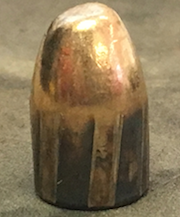
\includegraphics[width=1.58in]{./figure-static/bullet.png}
\includegraphics[width=3in]{./figure-static/striae.png}
\caption{%Photos depicting markings found on fired bullets.
(Top left) Traditionally rifled gun barrel. Grooves and lands alternate to give bullets a spin during the firing process.
Barrel create markings (striations) on a bullet when fired.
(Top right) Image of a fired bullet. The vertical stripes along the lower half of the bullet show groove and land engraved areas. The land engraved areas contain the microscopic striations created when the bullet passed through the barrel of the gun. (Bottom) Zoom into a land engraved area showing striations (vertical lines). }
\label{fig:bullet}
\end{figure}

\hh{In current practice, forensic firearm  examiners evaluate whether two bullets come from the same source (are fired from the same gun) or from different sources based on microscopic comparison of the striation patterns engraved on bullets during the firing process (see \autoref{fig:bullet}). }
\hh{This process is based on a visual and therefore subjective assessment of the evidence under a comparison microscope. }
%The discipline of firearm identification examines bullets to determine the likelihood that a bullet found in a criminal case was fired from a particular gun. To do this, the bullet from the crime will be compared with a bullet that was known to be fired from the gun under evaluation. When the bullet passes through the gun barrel, microscopic striations are created on the bullet as shown in \autoref{fig:bullet}. The dark vertical striped sections are called lands and are the regions where the striations are located. All of the bullets discussed in this paper have six lands. Markings on bullets fired from the same gun will have similar patterns, so these markings can be compared to determine if two bullets were fired from the same gun. Traditionally, this is a procedure that has been performed by hand. Specially trained examiners visually compare the bullet striations using a comparison microscope that allows the examiners to view both bullets at the same time \citep{nrc:2009}.
\hh{The lack of objective evaluation and the associated absence of established error rates has first been criticized by the National Research Council \cite{nrc:2009} and later by the President's Council of Advisors on Science and Technology \cite{pcast:2016}.}

%The scientific community has encouraged the inclusion of more data driven techniques to be used in forensic investigations \citet{nrc:2009}. These methods would allow for the reporting of a measure of uncertainty in addition to the conclusion drawn from the analysis. This led
In response \citet{hare:2016} proposed an automated machine learning method for bullet matching to complement a visual inspection by  firearm examiners.

\hh{Based on high-resolution topological scans of land engraved areas}
\citet{hare:2016} obtain signatures of  striations from   two bullet lands (\autoref{fig:signatures}). \hh{Features quantifying the similarity of signatures, such as the cross-correlation function, the distance between signatures, and the number of matching striae, are extracted and used to %variables that measure the similarity of the two signatures, and use a
train a random forest model to determine the probability of a comparison resulting from the same source (matching signatures) or from different sources (non-matching signatures).}

\begin{figure}[!t]
\centering
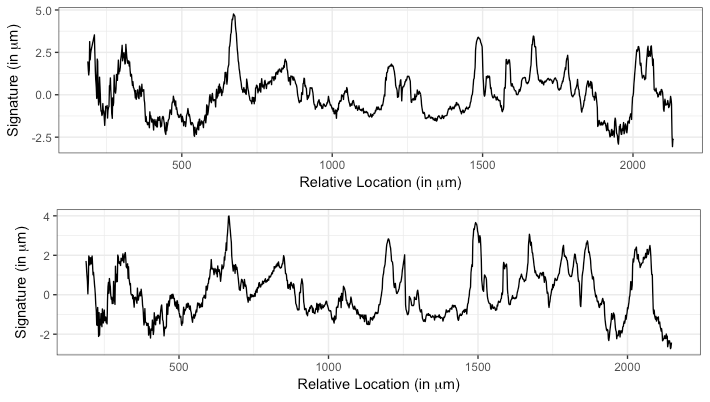
\includegraphics[width=3.5in]{./figure-static/signatures.png}
\label{fig:signatures}
\caption{Bullet signatures extracted from two bullets fired through the same barrel. The two signatures come from the same barrel-land and therefore have very similar patterns. The features used in the random forest from \citet{hare:2016} are different metrics that measure the similarity between two such signatures.}
\end{figure}




\hh{The random forest model trained in \citet{hare:2016} is available as object rtrees from the \emph{bulletxtrctr} R package. rtrees is trained on a set of scans obtained from one set of bullets of the James Hamby Consecutively Rifled Ruger Barrel Study \citep{hamby:2009} and based on 83028 land-to-land comparisons.}
The model was fit using nine features from the training data that measure the similarity between two bullet signatures (CCF, CMS, distance, distance standard deviation, matches, mismatches, non-CMS, rough correlation, sum of peaks), and the response variable (same source) is a binary variable indicating whether the two bullets were fired from the same gun (same source = TRUE) or not (same source = FALSE). Additional details about rtrees and definitions of the features are included in Appendix \ref{hamby-rf}.
\hh{XXX State the problem: we want to know how the model comes up with predictions. Random forest models are relatively simple for a Machine Learning method, but do not have readily available interpretations. RF models also are able to capture local and non-linear structures in the data.
XXX What are diagnostics statisticians would use in this case?
Generally, any method exploring multivariate relationships, such as a (generalized) scatterplot matrix would be a valid route.
Specific to Random Forest models would e.g. be importance of features and parallel coordinate plots.  }

\autoref{fig:bullet-plot-train} shows plots of the distribution of the proportion of same source across the range of each of the nine features. Many of the plots show a location within the range of the feature where the proportion land comparisons from the same source switches from FALSE to TRUE. This suggests that most of the variables are good predictors for determining whether two bullets are from the same source.

\begin{figure}[!t]
\begin{knitrout}
\definecolor{shadecolor}{rgb}{0.969, 0.969, 0.969}\color{fgcolor}
\includegraphics[width=0.5\textwidth]{figure/bullet-plot-train-1} 

\end{knitrout}
\caption{Distribution of the response variable \hh{explain the spine plots \cite{hummel:1996} a bit - they are non-standard}, same source, for the features used to fit the random forest rtrees. Each bin shows the proportion of land comparisons in the bin that are from the same source indicated by the color. Many of these variables have large ranges where the proportion of same source is either close to 0 or 1, which suggests that these features are good predictors of for determining whether two bullets are from the same source.}
\label{fig:bullet-plot-train}
\end{figure}

Another perspective of the rtrees training data is shown in \autoref{fig:bullet-plot-scatter}. The plots on the diagonal are histograms showing the univariate distributions of the variables. The plots on the off diagonal show the bivariate distribution of the response variable of same source. The feature space has been divided into a grid, and each cell is colored by the proportion of observations in the grid that are a comparison from the same source. Even in the bivariate perspective, there appears to be clear divisions between the bullet comparisons from the same source and different sources.

\begin{figure}[!t]
\begin{knitrout}
\definecolor{shadecolor}{rgb}{0.969, 0.969, 0.969}\color{fgcolor}
\includegraphics[width=0.5\textwidth]{figure/bullet-plot-scatter-1} 

\end{knitrout}
\caption{Bivariate visualizations of the rtrees training data. The plots on the off diagonal were created by dividing the feature space into a grid, and the color of each cell represents the proportion of observations in the cell that are from the same source. This shows clear divisions in the bivariate perspective between same source and different source comparisons based on the feature values. Additionally, histograms of the features are shown in the plots on the diagonal that depict the univariate distributions of the features.}
\label{fig:bullet-plot-scatter}
\end{figure}

\begin{figure}[!b]
\begin{knitrout}
\definecolor{shadecolor}{rgb}{0.969, 0.969, 0.969}\color{fgcolor}
\includegraphics[width=0.5\textwidth]{figure/bullet-plot-rfvi-1} 

\end{knitrout}
\caption{Variable importance plot for the random forest fit to the bullet matching dataset. The variables of rough correlation and CCF have the highest variable importance values followed by matches and mismatches.}
\label{fig:bullet-plot-rfvi}
\end{figure}

\begin{figure*}[!b]
\begin{knitrout}
\definecolor{shadecolor}{rgb}{0.969, 0.969, 0.969}\color{fgcolor}
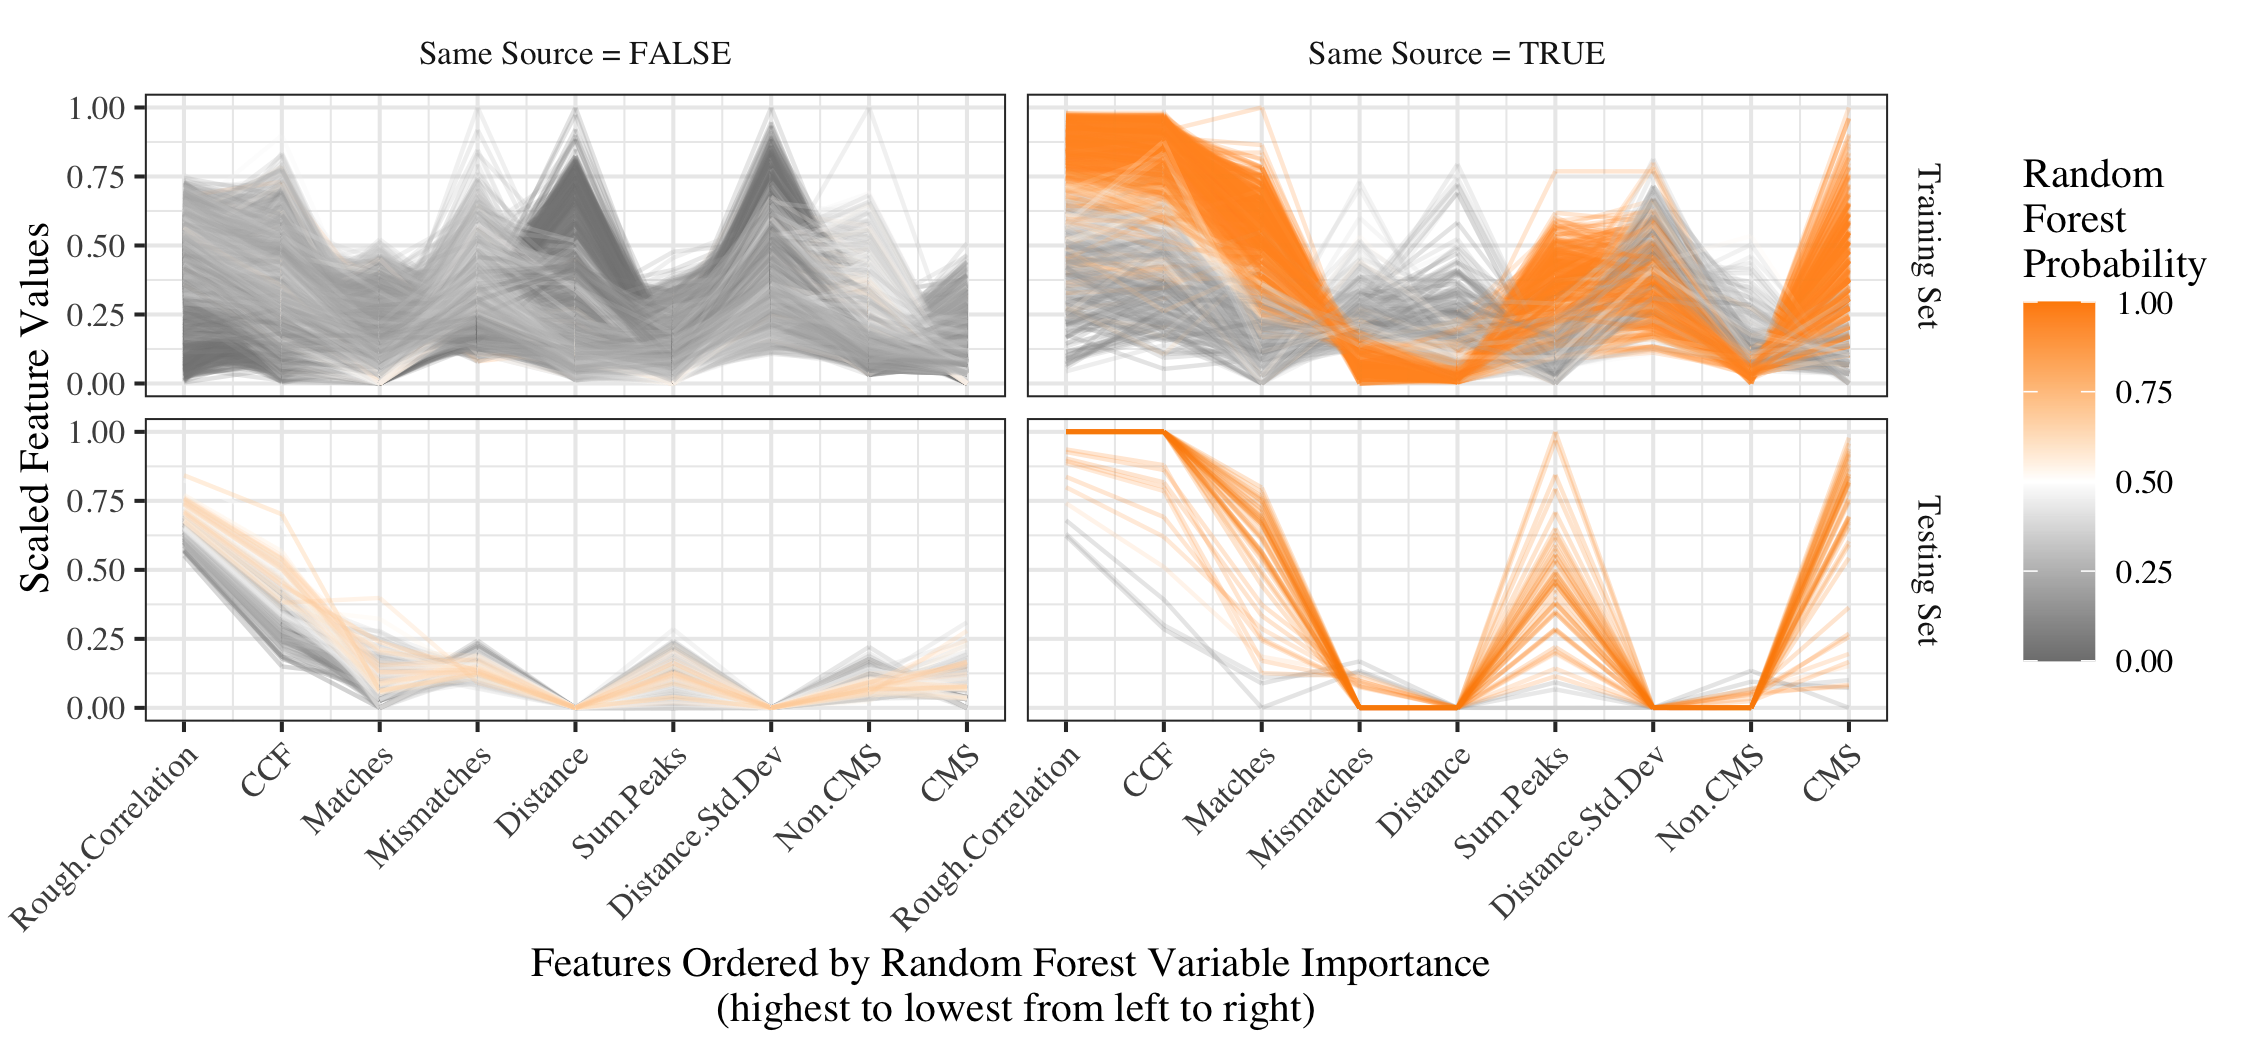
\includegraphics[width=\textwidth]{./figure-static/bullet_pcp} 

\end{knitrout}
\caption{Parallel coordinate plots of rtrees training and testing data. The training data are included in the plots on the top row, and the testing data are included in the plots on the bottom row. The left column contains the observations which are know to be comparisons of lands that are not from the same gun, and the known same source comparisons are on the right. The y-axis shows the standardized feature values, and the x-axis shows the features used to fit the random forest (ordered by feature importance). Each line corresponds to a comparison, and the color of the line represents the associated random forest probability. These figures show a clear relationship between the feature values and the probability returned by the random forest.}
\label{fig:bullet-plot-rfpcp}
\end{figure*}

\autoref{fig:bullet-plot-rfvi} shows the variable importance values produced by the rtrees. \kgc{KG: Look up what value is being used as the importance and describe it here.} Rough correlation and CCF have the highest variable importance values, and non-CMS and CMS have the lowest variable importance values.

rtrees was tested on another set of bullets from the Hamby study with 432 rows of land comparisons. \autoref{fig:bullet-plot-rfpcp} shows parallel coordinate plots of the rtrees training (top row) and testing (bottom row) datasets. The plots on the left contain comparisons know to be from from different sources, and the plots on the right contain comparisons know to be from the same source. Each line represents one observation in the data, and the color of the line represents the by the corresponding random forest probability. The standardized feature values are plotted on the y-axis, and the features are plotted on the x-axis, which are ordered from left to right from the highest to lowest random forest feature importance.

The majority of observations with random forest probabilities close to 1 have a clear pattern of corresponding feature values as can be seen in the plots where same source is known to be true. The observations where the random forest is wrong in returning high probabilities when same source is known to be true (i.e. same source is true but the random forest probabilities are between 0 and 0.5) have feature values that reflect those of observations where same source is known to be false as seen in the plots on the left. These plots provide insight into why the random forest is producing poor random forest probabilities for these observations.

Since firearm identification is commonly used as evidence for convictions in court cases, it is important to be able to understand and assess the model that is used to quantify the probability that a bullet was fired from a gun. An application of LIME to rtrees could provide an understanding of the key variables used by the random forest model to make a prediction. However, just as it is important to assess the random forest model for this high-stakes application, it is also important to assess the LIME explanations to make sure they are providing a trustworthiness understanding of the random forest model. We will apply LIME to rtrees and use our visual diagnostics to assess different implementations of LIME.

\subsection{Application of LIME to Bullet Matching Data}







\begin{figure*}[!th]
\begin{knitrout}
\definecolor{shadecolor}{rgb}{0.969, 0.969, 0.969}\color{fgcolor}
\includegraphics[width=\textwidth]{figure/bullet-feature-heatmap-1} 

\end{knitrout}
\caption{Feature heatmap of the 36 LIME implementations applied to the bullet comparison data test set. In addition to faceting the results by simulation method and order a feature was selected by LIME as done in \autoref{fig:sine-feature-heatmap}, this plot has been faceted by the Gower power and whether the the observation is from a match (TRUE) or non-match (FALSE). This plot shows several key insights about the LIME explanations. First, the features selected by LIME for the density simulation methods are mostly the same for all implementations and all cases. Second, the features selected by LIME for the bin based methods are affected by the number of bins but not the Gower power. Third, the explanations produced by LIME using bin based methods result in different important features for the matches and non-matches. \kgc{***Need to rotate the facet labels, so I can make the text bigger.}}
\label{fig:bullet-feature-heatmap}
\end{figure*}

It was of interest to see how the explanations from LIME varied across the all sampling methods with different Gower exponents when applied to the bullet matching data. LIME was applied to each prediction from the bullet test data obtained from the 'rtrees' random forest model for each of the four sampling methods (equally spaced bins, quantile bins, kernel density estimation, and normal approximation). For each of the bin based sampling methods, LIME was applied for 2 to 6 bins. It was decided to use 6 bins as the maximum, since the larger the number of bins, the more complex the explanation becomes. Each simulation method was implemented three times with Gower exponents of 0.5, 1, and 10. Thus, a total of $12\times 3=36$ different implementations of LIME were performed. These implementations of LIME were performed using our R package \emph{limeaid}. Each implementation was set to return 3 features by LIME and feature selection was performed using the highest weights method.

\subsection{LIME Assessment Visualizations}

\begin{figure*}[!t]
\begin{knitrout}
\definecolor{shadecolor}{rgb}{0.969, 0.969, 0.969}\color{fgcolor}
\includegraphics[width=\textwidth]{figure/bullet-lime-expls-1} 

\end{knitrout}
\caption{Plots of the LIME explanations associated with one observation in the bullet comparison test data from the implementations using 2 to 6 quantile bins. A bar chart showing the number of times a feature was selected by LIME in these five explanations is also included in the bottom right corner.}
\label{fig:bullet-lime-expls}
\end{figure*}

To get an overview of the LIME explanations from the 36 implementations, we consider our heatmap diagnostic plot for comparing the LIME implementations first shown in \autoref{fig:bullet-feature-heatmap}. The plot facets the features selected in the LIME explanations by the simulation method, the Gower power, the order the feature was chosen, and whether the observation is from a known match or non-match of bullet signatures. This plot highlights several key features of the LIME explanations from the bullet matching dataset.

First of all, the density simulation methods produced the same explanations for almost all cases and LIME implementation methods. As a result, the LIME explanations for the density implementation methods are global and not local. Second, within a bin based simulation method, the features selected by LIME for an observation often vary based on the number of bins used but do not appear to vary based on the Gower power used. Especially with the equal bin explanations, there are vertical stripes that suggest a dependence of the LIME explanations on the number of bins used. The vertical stripes are not as apparent with the quantile bins. Lastly, there are clear differences between the LIME explanations for the cases that are matches and those that are not matches which are produced by the bin based simulation methods. This provides evidence that suggests that the features which the random forests uses to classify a match are different from the features used by the random forest to classify a non-match.

The most important insight \autoref{fig:bullet-feature-heatmap} highlights is the dependence of the explanations on the LIME implementation method for many of the observations in the test data. To better understand how an explanation can vary based on the implementation method, we consider the explanations for one observation across several LIME implementations. The observation we consider from the bullet comparison test data is known to not be a match and has a random forest score of 0.05. \autoref{fig:bullet-lime-expls} shows the explanation plots from \emph{lime} for the LIME implementations using 2 to 6 quantile bins associated with this case from the test data. A bar chart showing the number of times a feature was chosen by one of these implementations is also included.

Rough correlation is the feature that appears the most in the explanations (4 out of 5 implementations). Distance and distance standard deviation are never selected. As the bar chart shows, 7 of the 9 features used to fit the random forest were selected at least once.by LIME. The set of features selected by LIME are different for each implementation except for 4 and 5 bins. However, the order in which the features are selected for the 4 and 5 bins differ, but the lengths of the bars for rough correlation and sum of peaks are very similar for both explanations. The $R^2$ values (indicated as the explanation fit in the figure) range from 0.032 (6 bins) to 0.35 (2 bins). The implementation with 2 bins has the best $R^2$ value, and this is the only explanation where the top feature contradicts a prediction of a match, which agrees with the random forest prediction that provides evidence that that two bullets are not a match. All of the other explanations have a top feature that supports a match, which does not agree with the random forest prediction. However, the second and third feature selected by LIME in the 2 bin case, support a match. Based on the variation in explanations across implementation and the features selected that support a match, which disagree with the random forest prediction, it is not clear which explanation to trust, if any.

\begin{figure*}[!t]
\begin{knitrout}
\definecolor{shadecolor}{rgb}{0.969, 0.969, 0.969}\color{fgcolor}
\includegraphics[width=\textwidth]{figure/bullet-metric-plot-1} 

\end{knitrout}
\caption{Plot of LIME assessment metrics for the 36 different implementations of LIME applied to the bullet comparison data test set. The shape of the points represents the power used for the Gower distance calculation, and the color of the points represents the rank associated with that observation within a metric. The density simulation methods perform well for all metrics, but the bin based metrics often do not agree in terms of performance across metrics.}
\label{fig:bullet-metric-plot}
\end{figure*}

To try to identify the LIME implementation method with the most trustworthy set of explanations, we created an assessment metric plot shown in \autoref{fig:bullet-metric-plot}. The three metrics of average fidelity, average $R^2$, and MSEE were computed for each of the simulation methods and Gower power used to implement LIME. The plot is faceted by the simulation method, and the shape of a point represents the Gower power. The color of a point represents the rank within a metric. That is, the darker a point, the better performance of that implementation method based on the metric.

The density simulation methods performed well across all implementation methods. This is an interesting result, since \autoref{fig:bullet-feature-heatmap} shows that the density methods results in global explanations. The metric values for the bin based implementation methods do not agree across metrics. For example, 2 and 3 quantile bins performed well according to the average $R^2$ but poorly according to MSEE. As a result, with the bin based methods, it is difficult to know which method to recommend. When considering the metrics across the Gower power used, the implementations using a power of 0.5 perform best or as well as the other powers in across all simulation methods. This suggests that the power that leads to a more global explanation is preferred by LIME in this example.

Unfortunately, \autoref{fig:bullet-feature-heatmap} leaves us without a clear indication of which set of explanations to use to explain the random forest. Perhaps we can say that the kernel density method, 3 equal bins, and 3 quantile bins are some of the best performing methods. To better understand the explanations provided by these three methods, we take a closer look at explanations from these methods for two observations of interest where one is a known non-match (case 20) and the other is a known match (case 325).

Figures \ref{fig:bullet-eois-nonmatch} and \ref{fig:bullet-eois-match} contain plots that provide this closer look for the known non-match and match, respectively. The top row of plots in each figure are the explanation plots from \emph{lime}. The bottom row of plots show scatterplots of the features selected by LIME colored by the random forest model prediction. The location of the prediction of interest is indicated on the scatterplots by a diamond, and black solid lines are included on the plots representing the bin divisions for implementations using bins. The bottom row plots are created using \emph{limeaid}. The plots within a column are associated with one of the three implementation methods (kernel density, 3 equal bins, or 3 quantile bins).

The scatterplots provide a visualization that helps to explain the LIME explanation. For example, consider the explanation for case 20 when 3 quantile bins were used. The explanation plot from \emph{lime} shows that case 20 having an observed CCF value greater than 0.320 supports a random forest prediction in favor of a match. The scatter plots show that many of the simulated values with CCF greater then 0.320 have random forest predictions greater than 0.5. Additionally, the LIME explanation indicates that a value of matches less than or equal to 1.66 contradicts a prediction in favor of a match. The scatter plots shows that almost all simulated values with a value of matches less than or equal to 1.66 have random forest predictions close to 0. Similar statements can be made about the 3 equal bin explanation for this case and the bin based implementations for the known match observation explanations. \kgc{**Consider creating a different set of plots for the kernel density (and normal approximation) methods that plot the rfscores versus the features and include the model.}

While the scatterplots provide visual explanations for the LIME explanations, some of them indicate that LIME falls short of a good explanation of the random forest predictions. Again, consider the explanation for case 325 when 3 quantile bins were used. From looking at the scatter plot of CCF versus matches, a better explanation for the random forest prediction would be to say that because the prediction of interest has a value of CCF less than 0.8 (approximately) and a value of matches less than 7 (approximately), the random forest is providing a prediction that supports a non-match. The relationship between ccf and rough correlation does not provide much evidence to support the random forest prediction one way or the other due to the mixture of random forest predictions ranging from 0 to 1 in most regressions, but there is a pentagon shaped region at the bottom of the scatter plot of matches versus rough correlation that the prediction of interest falls in that supports the random forest prediction of a non-match.



\begin{figure*}[!htbp]
\begin{knitrout}
\definecolor{shadecolor}{rgb}{0.969, 0.969, 0.969}\color{fgcolor}
\includegraphics[width=\textwidth]{figure/bullet-eois-nonmatch-1} 

\end{knitrout}
\caption{Plots of LIME explanations for one case in the test data that is a known non-match. Each column contains plots associated with a different implementation (3 quantile bins, 3 equal bins, or kernel density). The top row of plots are the explanation plots from \emph{lime}. The bottom row shows scatter plots of the simulated data associated with the prediction of interest. The features plotted are those chosen by LIME in the explanations, and the points are colored by the the random forest predictions. Lines showing the divisions created in the feature space by the bin based LIME methods are included as solid black lines. The scatter plots can be used to better understand the LIME explanation and assess if it is a good explanation.}
\label{fig:bullet-eois-nonmatch}

\vspace*{\floatsep}

\begin{knitrout}
\definecolor{shadecolor}{rgb}{0.969, 0.969, 0.969}\color{fgcolor}
\includegraphics[width=\textwidth]{figure/bullet-eois-match-1} 

\end{knitrout}
\caption{Plots with the same structure as \ref{fig:bullet-eois-match} but for an observation from the test data that is a known match.}
\label{fig:bullet-eois-match}
\end{figure*}

The scatter plots of the kernel density implementations for both the match and non-match case show that almost all of the simulated values have random forest predictions less than 0.5, which provide evidence in favor of a non-match. It appears that simulation method is not providing enough values to cover the feature space that hit regions where the random forest provides predictions above 0.5. The training data has a much smaller amount of matches (1221) than non-matches (81807), and this simulation method is clearly affected by this imbalance in the two classification categories. Furthermore, this may be the cause of the minimal amount of variability in the LIME explanations across all of the cases in the test data.

Without applying multiple implementations LIME to the bullet test data or viewing diagnostic plots of the LIME explanations, it may be very possible to formulate reasons why the LIME explanations make sense. However, the sequence of plots in this section (Figures \ref{fig:bullet-feature-heatmap}, \ref{fig:bullet-lime-expls}, \ref{fig:bullet-metric-plot}, \ref{fig:bullet-eois-match}, and \ref{fig:bullet-eois-nonmatch}) suggest that we should be cautious to trust any of these LIME explanations. While some of them provide an explanation that may be reasonable, there could be better explanations (as seen in the 3 quantile bin case of \autoref{fig:bullet-eois-match}), and some of them provide explanations that make no sense (as seen in \autoref{fig:bullet-lime-expls}). It appears that either LIME needs to be further tuned to provide trustworthy and good explanations, or a different approach may provide better insight. As glimpsed with the scatter plots in Figures \ref{fig:bullet-eois-match} and \ref{fig:bullet-eois-nonmatch}, the more traditional approach to explanation random forest predictions by plotting the random forest predictions over the feature space (partial dependence plots), could provide better insight into the complex model with no need to assess the explanation method if the sampling method is well chosen.

\section{Discussion} \label{discussion}

\kgc{Need to add a discussion on using our visualizations in situations without tabular data or a dichotomous response variable.}\\
\\
In this paper, we have presented visualizations that depict the steps in the LIME algorithm (\autoref{procedure}) and diagnose LIME explanations (Sections \ref{set-visuals} and \ref{implementation-visuals}). Our intentions with these visualizations were to provide insight on how LIME works, assess the ability of the explainer model to capture the complex predictive model, and compare LIME explanations produced by different tuning parameters. While the visualizations accomplish these tasks, they also expose examples of the failings of LIME. To address the discovered failings of LIME, we will reconsider each of the claims about the performance of LIME made by \citep{ribeiro:2016} (interpretability, faithfulness, linearity, and localness) in light of the insights gained from the diagnostic visualizations.

As previously discussed, the \textbf{interpretability} of the LIME explanations can be controlled by the complexity of the explainer model. For example, the number of bins selected for simulation can control the interpretability of the explanations. If too many bins are selected, the bin range that is reported in the LIME explanation will be too small to be meaningful in the context of the feature. An appropriate choice of the number of bins will keep the bin range meaningful. Thus, the claim of interpretability does not need to be assessed using the visualizations. However, diagnostic visualizations do present a different perspective on the meaning of interpretability.

\kgc{**Need to rework this paragraph and the next two. The ideas are here, but they are worded very poorly.} Even though an explanation will be interpretable as long as the complexity of the explainer model is appropriately chosen, the presentation of a LIME explanation in the key visual used by \citep{ribeiro:2016} (shown in \autoref{fig:sine-plot-poi}) could lead to an over simplified interpretation of the explainer model. Without a solid understanding of the details behind the fitting of the explainer model, the deeper meaning of the bars in the figure is lost.

It is customary to interpret this plot by stating that the direction of the bar supports or contradicts the classification in a certain category, and the length of the bar signifies the importance of the involvement of a feature in the prediction. While these interpretations are correct, the lengths of the bars represent the coefficients of the ridge regression model used as the explainer model, which contain more meaning than just the direction of support and importance of a feature. The bars indicate how much the average complex model prediction estimated by the linear explainer model changes based on a change in the feature. Furthermore, this interpretation changes depending on whether a bin based or density simulation method was used (i.e the change in the average complex model prediction between an observation in the same bin as the case of interest and an observation not in the same bin versus the change in the mean complex model prediction for a change in the feature by one standardized unit).

Thus, even though an explainer model may be interpretable, the explanation it produces may be under-interpreted or misinterpreted without an understanding of the process that produced the explanation. Supplementing \citep{ribeiro:2016}'s compact visualization of the explanation with visualizations of the explanation that depict the simulated data and the explainer model (such as Figures \ref{fig:sine-plot-step3ab} and \ref{fig:bullet-eois-match}) promotes a full interpretation of the explanation. This is done by providing reminders of the meaning of the lengths of the bars in addition to a visual connection between complex model predictions and the estimated coefficients of the explainer model.

Even with an explainer model that is interpreted correctly, the interpretation is worthless if the explainer model is not \textbf{faithful} to the complex model. This claim can be easily assessed using the diagnostic plots suggested in this paper. Many of the visualizations in this paper highlight problems with the faithfulness of the explainer models.

The visualizations that incorporate the bins along with the complex model predictions (Figures \ref{fig:fig:sine-plot-step1ab}, \ref{ fig:sine-plot-step1c}, \ref{fig:sine-plot-step3ab}, \ref{fig:sine-plot-compare-bins}, \ref{fig:bullet-eois-match}, and \ref{fig:bullet-eois-nonmatch}) highlight issues that accompany the choice to use bin based simulation methods. These visualizations allow for a comparison of the size of the bins to the complex model's decision boundaries. All of the examples in this paper show cases where the bins do not accurately capture the classification boundaries near the predictions of interest of the random forest models by oversimplifying the model. Using less bins would clearly not help improve the faithfulness of the explainer model in these examples, and while an increase in bins would lead to a finer resolution of the random forest classification boundaries, interpretability of the explainer model would quickly be lost. The bins used by LIME are not flexible enough to capture the different sized division boundaries of the random forests shown in this paper. Perhaps this could be improved by allowing the bin creation to account for the relationships between the features and response variable or a different number of bins for each feature.

The figures referenced in the previous paragraph from the \data \ example are all based on the implementation of LIME using a set of tuning parameters. From the use of the feature heatmap, we found that different sets of tuning parameters can produce different explanations. It makes sense that one set of tuning parameters could lead to a more faithful explainer model than another. As a result, we proposed a visual comparison of two faithfulness metrics (MSEE and average fidelity). The examples of faithfulness metric comparisons in this paper (Figures \ref{fig:sine-metric-plot} and \ref{fig:bullet-metric-plot}) both produced confusing results. In both examples, the density based simulation methods resulted in the best or close to the best performance even though the feature heatmaps (Figures \ref{fig:sine-feature-heatmap} and \ref{fig:bullet-feature-heatmap}) showed that the density simulation methods produced global explanations with no variation in features selected by LIME. For the bin based simulation methods, the two metrics often did not agree or contradicted one another, which makes it difficult to decide on a recommendation of a set of tuning parameters that produces the explanations with the most faithful explainer model.

The metric comparison plot also includes a comparison of average $R^2$ values, which is a metric that can be used to assess the claim of \textbf{linearity}. Most of the average $R^2$ values in the examples from this paper are below 0.5 suggesting a poor linear fit of the explainer models. The poor linear fit of the explainer model was also seen with the residual plot (\autoref{fig:sine-plot-step2cd}).

The final claim, \textbf{localness}, is also addressed by the feature heatmap and metric comparison plot. As stated, the feature heatmap revealed that the density simulation methods in the examples of this paper resulted in global explanations where the same features were repeatedly chosen across all (or almost all) observations in the set of explanations. This finding agrees with that of \citep{laugel:2019} who also found LIME produced global explanations with the normal approximation simulation method. For the bin based simulation methods in the bullet data example, the feature heatmap showed that the features chosen for the explanations varied between the two classification categories (match versus non-match). This is an interesting finding that suggests that different features can play a role in the predictions of observations in different response categories, but the patterns of features selected by LIME within a classification category do not vary. Again, this is a suggestion of global explanations. Furthermore, while the metric comparison plot in the bullet example did not provide agreement between metrics on a best bin based method, all metrics agree that a Gower power of 0.5 for computing the model weights associated with distance of a simulated data point from the prediction of interest was best. This suggests that a less local explanation provided a better explanation of the performance of the random forest.

Some of the visualizations in the paper generalize easily to any application of LIME such as the feature heatmap and metric plot. Other plots such as the visualizations of the LIME procedure would require extensions such as the use of scatterplot matrices to compare explanations with more than two features. The addition of interactivity to the diagnostic plots would provide additional enhancement of the assessment process. For example, a diagnostic plot that provides a summary of multiple LIME explanations, such as the feature heatmap, could be displayed and clicked on to reveal more detailed figures associated with individual predictions of interest, such as plots of the simulated data and explainer model.

While it would be ideal if LIME could be used as a method to provide easily understandable explanations for black-box models as \citep{ribeiro:2016} claim, that dream is not yet a reality. The examples using diagnostic plots to assess LIME in this paper show frequent issues with LIME. The practice of assessing the performance of methods has once again shown its importance. We hope that our plots provide motivation to assess LIME explanations, to not blindly use the default settings (even if it is not clear which tuning parameters to use), and perhaps to encourage work on improving LIME, so that it can be a lime and not a lemon.

\kgc{Need to work this into the discussion: We acknowledge that not all prediction problems will produce trends as easy to interpret as the visualizations we have shown in the section, but we still believe that visualizations of the procedure can provide insight into the quality of the LIME explanation. We hope these figures will provide a starting point (if not an ending point) for the assessment of a single LIME explanation. Perhaps the inability to interpret a plot is itself telling, or the act of creating extensions of these visualizations to work with a different scenarios will lead to an understanding of the trustworthiness of the explanation.}

\section*{Acknowledgments}

This is acknowledgment text. Provide text here.

\subsection*{Author contributions}

This is an author contribution text. This is an author contribution text. This is an author contribution text. This is an author contribution text. This is an author contribution text.

\subsection*{Financial disclosure}

None reported.

\subsection*{Conflict of interest}

The authors declare no potential conflict of interests.

\section*{Supporting information}

The following supporting information is available as part of the online article:

\appendix

\section{Additional Details on the LIME Procedure as Implemented in R} \label{lime}

\kgc{Just copying text here for now...}\\
\\
\textbf{Data Simulation}\\
\\
The density approximation method leaves the continuous features in their original form and then approximates the density of each feature using either a kernel density estimator or a normal distribution with mean and standard deviation equal to the sample mean and standard deviation of the observed feature values. The density approximation methods will be referred to as kernel density approximation and normal approximation, respectively. For both methods, observations for $\textbf{X}^*$ are sampled from the estimated distributions.\\
\\
\textbf{Interpretable Transformation}\\
\\
The interpretability transformation that corresponds to the density approximation simulation methods standardizes all of the observations by subtracting the feature sample mean and dividing by the feature sample standard deviation.\\
\\
\textbf{Explainer Model}\\
\\
\hh{XXX The next couple of paragraphs are hard to read - they are quite abstract and and full of technical details. You could try to show the visualization first, and then go into a precise discussion of why the weights are not decreasing as you'd expect by going into this discussion. That has the benefit of motivating the reader to actually read through the details and highlights your work over LIME.  XXX}

For the computation of the weights, \emph{lime} allows for the use of the Gower distance \citep{gower:1971} or an exponential kernel. If the Gower distance is used, the weights are computed prior to the interpretability transformation by computing the Gower similarity metric raised to some power. That is, let observation $z'_i$ have weight $\omega_{x^*}(\textbf{x}'_i) = Gower(x^*, x'_i)^c$, where $Gower$ represents the computation of the Gower similarity and $c$ is some constant. This denotes a proximity measure between $x^*$ and $x'_i$ for each $i\in 1,...,m$. If the exponential kernel is used, the weights are computed after the interpretability transformation such that $z'_i$ has weight $\omega_{z^*}(\textbf{z}'_i)$. \kgc{Could change weight notation to $|| \cdot ||$.}

The process to obtain the explainer model involves two steps. First, feature selection is performed to identify the $P$ most important variables in the local region where $P$ is specified. \emph{lime} offers several options for performing feature selection. These options are as follows where all methods are applied to $\textbf{Z}'$ with weights of $\omega_{z^*}(\textbf{z}'_i)$.
\begin{itemize}
\item Forward Selection: Forward selection is performed using a ridge regression model with a shrinkage parameter of $\lambda=0$ to select $P$ features.
\item Highest Weights: A ridge regression model with a shrinkage parameter of $\lambda=0$ is fit using all $p$ features. The $P$ features with the largest coefficients in the ridge regression are selected.
\item LASSO: A LASSO model is used to select the $P$ features.
\item Classification Tree: A classification tree is fit. The first $P$ features used as breaks in the tree are selected.
\end{itemize}
The ridge regression and LASSO models are fit using the \emph{glmnet} package in R \citep{simon:2011}. By default, \emph{glmnet} standardizes all predictor variables prior to fitting a model, but the coefficients are returned on the original scale.

\hh{shorten}
Both the proximity metric and the type of feature selection \sout{used could} have an effect on the LIME explanation, so it is of interest to visualize this part of the LIME process. By default, \emph{lime} uses the Gower distance with $c=1$.
\hh{shorten-end}

The second \hh{and final} step in fitting the explainer model is to fit a ridge regression model to the selected features.

\hh{XXX results first, then the technical details. There's actually more indices in the model than different prediction results. LIME hides this simplicity behind a wall of technical details. Don't help them with it.}

Define the subset of $\textbf{Z}'$ containing the chosen $P$ features as $\textbf{Z}'_P$. A ridge regression model is fit using \emph{glmnet} to $\textbf{Z}'_P$ with $f\left(\textbf{X}'_P\right)$ as the response vector, a shrinkage parameter of $\lambda=2/n$ \kgc{(KG: Note that *lime* updated lambda in ridge regression final model)}, and weights of $\omega_{x^*}(\textbf{x}'_i)$ or $\omega_{z^*}(\textbf{z}'_i)$ depending on the simulation method used as discussed in \autoref{step1}. This ridge regression is used as the explainer model $g$. For the remainder of the paper, let
  $$g\left(\textbf{Z}'_{P}\right)=\hat{\beta}_0+\hat{\beta}_1z'_{1}+\cdots+\hat{\beta}_Pz'_{P}$$
where $\hat{\beta}_0, \hat{\beta}_1,...,\hat{\beta}_P$ are the estimated coefficients from the ridge regression.

The explainer model fit by \emph{lime} for the prediction of interest from the \data \ example is written as

$$g\left(\textbf{Z}'_{2}\right) = 0.5-0.1I\left[x_1\in (-0.3, 4.8] \right]+0.3I\left[x_2\in (4.8, \ensuremath{\infty{}})\right].$$

In terms of feature selection, \emph{lime} performs forward selection by default if the number of features requested to be selected is 6 or less, as in the case of the \data. If more than 6 features are specified to be selected, then the highest weights method is used. \\
\\
\textbf{Interpretation}\\
\\
 In the case of density approximation samples, the features used to fit $g$ have been standardized. Again the magnitudes of the coefficients indicate the importance of the features, but a coefficient can be interpreted as the amount the response probability increases/decreases for an increase in one unit of feature $j$.

\section{Procedure Visualizations with Three Features} \label{scatter-plots}

Section \ref{procedure} describes visualizations of the LIME procedure for the features of $x_1$ and $x_2$ of the \data. The feature of $x_3$ was excluded from visualizations since it was not one of the two features selected by LIME for the explanation of the prediction of interest. However, it may be of interest to incorporate $x_3$ in the visualizations of the the steps of the LIME procedure that include. These visualizations are shown in Figures \ref{fig:app-plot-step0} through \ref{fig:app-plot-step2a}. Note that the inclusion of $x_3$ in visualizations after feature selection is not necessary, and the visualizations would remain the same as shown in Section \ref{procedure}, so they are not included here. Figures \ref{fig:app-plot-step0} and \ref{fig:app-plot-step1a} show plots of the training and testing data that make it clear that there is a relationship between the response variable and $x_1$ and $x_2$ but no relationship between the response and $x_3$. \autoref{fig:app-plot-step1b} shows the discretization of the features from the interpretability transformation. Lastly, \autoref{fig:app-plot-step2a} highlights that the value of $x_3$ is taken into account when assigning weights to the simulated data.

\begin{figure*}[!t]
\begin{knitrout}
\definecolor{shadecolor}{rgb}{0.969, 0.969, 0.969}\color{fgcolor}
\includegraphics[width=\textwidth]{figure/app-plot-step0-1} 

\end{knitrout}
\caption{Scatter plots of all features from the \data \ training (top) and testing (bottom) sets. The points are colored by the observed response and the random forest probability, respectively. The prediction of interest is indicated by a diamond. There is a clear relationship between the response and $x_1$ and $x_2$ but no relationship between the response and $x_3$.}
\label{fig:app-plot-step0}
\end{figure*}

\begin{figure*}[!t]
\centering
\begin{knitrout}
\definecolor{shadecolor}{rgb}{0.969, 0.969, 0.969}\color{fgcolor}
\includegraphics[width=\textwidth]{figure/app-plot-step1a-1} 

\end{knitrout}
\caption{Scatter plots of all features from the \data \ training set (top) and the four quantile bin simulated data (bottom). All sets are overlaid with black lines depicting the four quantile bins.}
\label{fig:app-plot-step1a}
\end{figure*}

\begin{figure*}[!t]
\centering
\begin{knitrout}
\definecolor{shadecolor}{rgb}{0.969, 0.969, 0.969}\color{fgcolor}
\includegraphics[width=\textwidth]{figure/app-plot-step1b-1} 

\end{knitrout}
\caption{\kgc{I'm still thinking about how to visualize all three features for the discretization step, but here is my starting point.}}
\label{fig:app-plot-step1b}
\end{figure*}

\begin{figure*}[!t]
\centering
\begin{knitrout}
\definecolor{shadecolor}{rgb}{0.969, 0.969, 0.969}\color{fgcolor}
\includegraphics[width=\textwidth]{figure/app-plot-step2a-1} 

\end{knitrout}
\caption{Hex plots of the weights assigned to the observations in the simulated data for each pair of features in the \data. The color of each hexagon represents the average weight of the points located within that region.}
\label{fig:app-plot-step2a}
\end{figure*}

\section{Details of the Bullet Matching Random Forest Model} \label{hamby-rf}

\bibliography{references}

% Do I need to include this?
% \section*{Author Biography}
% \begin{biography}
% {\includegraphics[width=60pt,height=70pt,draft]{empty}}
% {\textbf{Author Name.} This is sample author biography text this is sample author biography text}
% \end{biography}

% \newpage
% 
% \textsc{\textbf{Ideas for describing proposed plots}}
% 
% \begin{itemize}
% \item start at the high level explanation (this is what we want to do and this is how we do it)
% \item go over a good and bad example
% \item include schematics of the plot first (good and bad) and then include the sine mini example version
% \item explain the expectation of the plot
% \end{itemize}
% 
% \textsc{\textbf{Comments for Editing}}
% 
% \begin{itemize}
% \item \hh{Generally: avoid 'can be'. Replace by 'is'.  }
% \item \hh{References like 'they', 'them' ... replace them by repeating the noun you are referring to to avoid any kind of ambiguity}
% \item \kgc{words to go back and make sure I am not using too often: ability, produce, understand}
% \item \kgc{decide on features or predictor variables}
% \item \hh{it's tuning parameters, not tunning} \kgc{Oops! I get that one wrong all of the time}
% \item \kgc{Adjust text sizes in plots so they all match}
% \item \kgc{Color scheme - comment from Heike:} \hh{I like the red-blue scheme for binary values, I also like the color scheme in the features heatmap. Generally papers and color don't go well together anyways, but we will solve that problem when we have to ... Most likely we will have to just pay the extra color fee}
% \item \kgc{Check that I am consistently referring to the perturbing as data simulation}
% \item \kgc{Clean up notation}
% \item \kgc{Referring to the linearity assumption:} \hh{Be a bit careful in the phrasing here - we can always approximate any function using a linear form (think Taylor expansion). The question is how big the error is.}
% \item \kgc{Make sure plots in the same figure are the same size}
% \item \kgc{Make sure I am distinguishing between RF predictions and probabilities correctly}
% \item \kgc{Use prediction of interest not case of interest}
% \item \kgc{Make sure I always treat the word 'data' as plural}
% \item \kgc{dataset or data set?}
% \item \kgc{scatterplot or scatter plot (check other plot names as well)}
% \item \kgc{choose whether to use the term feature or variable and make sure it is consistent throughout}
% \item \kgc{just include the details about LIME that are necessary to understand the plots and remove the rest to the appendix}
% \item \hh{avoid the use of implicit references like `this' and `that'. Make the reference explicit by adding what you are referring to, such as `this method', `that procedure'}
% \item \hh{make sure to use exact phrases. things like `LIME was developed in 2016' is factually questionable - but we know LIME was introduced in 2016. Also `the authors were interested in ...' implies that you know their intent. It's better to not guess any intent but stick to what we know.}
% \item \hh{`our` diagnostics ... you are using `our` quite often. It is good to claim work, but it is not good to claim things that we want others to use, because that is by definition excluding everybody but you. It's better to re-phrase with a focus on what you did. We introduce, we suggest, etc.}
% \item \hh{Try to give each of the diagnostics a name.}
% \item \kgc{check that I am always using present tense}
% \item \kgc{check that I am consistent in my use of the term black-box model}
% \end{itemize}
% 
% \textsc{\textbf{Ideas for Publishing}}
% 
% \begin{itemize}
% \item longer review article (emph on CS method in ML - we're translating the content into a stats language) (talk to Maitra and Wendy)
% \item review article would need a more extensive lit review:
% \begin{itemize}
% \item who has looked at LIME and found it not great
% \item who is using LIME for applications
% \item papers using LIME
% \end{itemize}
% \item the diagnostics plots could get put in a rapid research paper via DS journal
% \item could consider JOSS for publication of the limeaid package
% \item implement a hierarchical ordering method for the feature heatmap
% \end{itemize}
% 
% \textsc{\textbf{Other Ideas}}
% 
% \begin{itemize}
% \item Consider creating a plot to show the decay of the distance by Gower exponent in terms of standard deviations in the appendix.
% \end{itemize}

\end{document}
